% draft会跳过文档中的所有图片。正式导出时需要删掉draft参数。
\documentclass[12pt, a4paper, oneside]{ctexart}

\usepackage{amsmath}
\usepackage{amssymb}
\usepackage{bm}
\usepackage{graphicx}
\usepackage{mathrsfs}
\usepackage{geometry}
\usepackage{framed}
\usepackage{color}
\usepackage{caption}
\usepackage{listings}
\usepackage{fancyhdr}
\usepackage{booktabs}
\usepackage{makecell}
\usepackage{indentfirst}
\usepackage{authblk}
\usepackage{multicol}
% \usepackage{draftwatermark}       % 需要应用水印时取消注释
\usepackage{enumitem}
\usepackage[hidelinks]{hyperref}
\usepackage{tikz}
\usetikzlibrary{positioning, shapes.geometric}

% 分栏线宽
\columnseprule=0.4pt

% 定制第二级无序列表的点样式
\setlist[itemize,2]{label=$\diamond$}

\pagestyle{fancy}

\fancyhf{}      % 清空页眉页脚设置
\fancyhead[L] {
    % 工大计算机系logo
    
\includegraphics[height=7mm]{./images/logo1.jpg}
}
\fancyhead[C]{《计算机网络》复习}
\fancyhead[R]{\leftmark}    % 右侧页眉:当前章标题

% 页脚居中放置页码
\fancyfoot[C]{\thepage}

% 设置章节标题自动编号的格式
\ctexset{
  section/number=\chinese{section},
%   subsection/name={,},
%   subsection/number=\chinese{subsection}
}

% 行距。ctexart默认值为1.3
\linespread{1.2}

\lstset{
  language=pascal,
  basicstyle=\ttfamily,
  frame=single,
  numbers=left
}

% \SetWatermarkText{Eslzzyl整理}            % 设置水印内容
% \SetWatermarkLightness{0.9}             % 设置水印透明度 0-1
% \SetWatermarkScale{0.8}                   % 设置水印大小 0-1

\renewcommand{\headrulewidth}{1pt}  %页眉线宽,设为0可以去页眉线
\renewcommand{\footrulewidth}{1pt}  %脚注线的宽度

\definecolor{shadecolor}{RGB}{241, 241, 255}

\title{
    
\includegraphics[width=0.3\textwidth]{images/hfut-badge.pdf}
    
    \vspace{20pt}
    《计算机网络》总复习
}
\author{Eslzzyl}
\date{\today}

\newcounter{problemname}
\newenvironment{problem}{\begin{shaded}\stepcounter{problemname}\par\noindent\textbf{例题\arabic{problemname}. }}{\end{shaded}\par}
\newenvironment{solution}{\begin{shaded}\par\noindent\textbf{解答:}}{\end{shaded}\par}
% \newenvironment{solution}{\par\noindent\textbf{答案. }}{\par}
% \newenvironment{note}{\par\noindent\textbf{例题\arabic{problemname}的注记. }}{\\\par}
\newenvironment{note}{\par\noindent\textbf{注记. }}{\par}

\begin{document}

\maketitle
\newpage
\tableofcontents
\vspace{20pt}
% 如果在目录处有备注,可以写在这里。

\newpage

\section{计算机网络体系结构}

\subsection{计算机网络概述}

\subsubsection{计算机网路的概念}

定义(周健PPT):将若干台具有\textbf{独立}功能的计算机系统,用某种或多种通信介质连接起来,通过完善的网络协议,在\textbf{数据交换}的基础上,实现网络\textbf{资源共享}的系统称为计算机网络。 

\begin{itemize}
    \item 独立:每台计算机都可运行各自独立的操作系统,彼此地位平等,无主从之分。
    \item 数据交换是网络的最基本功能。
    \item 资源共享是网络最终目的。
\end{itemize}

\subsubsection{计算机网络的组成}

\begin{itemize}
    \item 从组成部分上看
    \begin{itemize}
        \item 硬件:主机(端系统)+通信链路+交换设备+通信处理机+……
        \item 软件
        \item 协议
    \end{itemize}
    \item 从工作方式上看
    \begin{itemize}
        \item 边缘部分:即用户使用的主机
        \item 核心部分:由路由器连成的交换网络
    \end{itemize}
    \begin{figure}
        \centering
        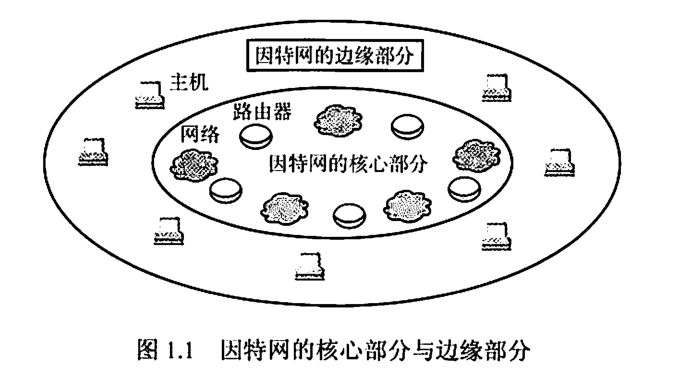
\includegraphics[width=0.8\textwidth]{./images/network_core_and_edge.png}
    \end{figure}
    \item 从功能组成上看
    \begin{itemize}
        \item 通信子网:由路由器和通信链路构成。
        \item 资源子网:由连接到通信子网的服务器和主机构成
    \end{itemize}
\end{itemize}

\subsubsection{计算机网络的功能}

五大功能:
\begin{enumerate}
    \item 数据通信:最基本的功能。
    \item 资源共享:是软件、数据、硬件的共享,提高这些资源的利用率。
    \item 分布式处理:将单一计算机的负荷分摊给其他计算机,利用空闲资源,提高系统利用率。
    \item 提高可靠性:多台机器可以通过网络相互替代。
    \item 负载均衡:将负载均衡地分配
\end{enumerate}

\subsubsection{计算机网络的分类}

\begin{enumerate}
    \item 按分布范围分类
    \begin{itemize}
        \item 广域网(WAN):数百公里以上。最大的广域网是Internet
        \item 城域网(MAN):覆盖一个大城市,大约几十到上百公里。
        \item 局域网(LAN):覆盖大楼、校园或厂区,不超过数公里。
        \item 个人区域网(PAN):就是个人热点
    \end{itemize}
    如果CPU的距离非常近(<1m),那么一般认为是多处理器系统而非网络。
    \item 按传输技术分类
    \begin{itemize}
        \item 广播式网络:多用于局域网,也用于广域网中的无线、卫星通信。
        \item 点对点网络:广域网基本上都是点对点的。
        \item 二者的重要区别在于是否使用存储转发、路由选择机制。若是,则属于点对点网络。
    \end{itemize}
    \item 按拓扑结构分类
    \begin{itemize}
        \item 总线形网络:建网方便,但高负载时效率低下,总线对故障敏感
        \item 星形网络:依赖中央设备
        \item 环形网络:典例:令牌环局域网
        \item 网状网络:多用于广域网。又可分为:
        \begin{itemize}
            \item 规则形网络
            \item 不规则形网络
        \end{itemize}
    \end{itemize}
    \begin{figure}
        \centering
        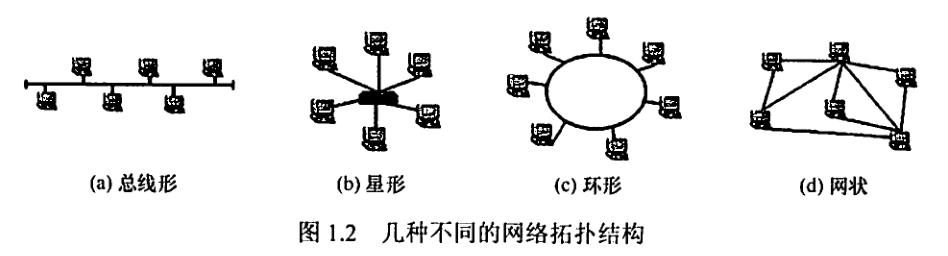
\includegraphics[width=0.8\textwidth]{./images/topo_structures.png}
    \end{figure}
    \item 按使用者分类
    \begin{itemize}
        \item 公用网:电信公司出资建造的大型公用网络
        \item 专用网:特定机构建立的专有网络
    \end{itemize}
    \item 按交换技术分类
    \begin{itemize}
        \item 电路交换网络:包括建立连接、传输数据和断开连接三个阶段。
        \begin{itemize}
            \item 优点:数据直接传送,时延小,实时性好。
            \item 缺点:线路利用率低,不便于差错控制。
        \end{itemize}
        \item 报文交换网络:存储转发整个报文
        \begin{itemize}
            \item 优点:线路利用率高
            \item 缺点:资源开销和时延都增大。
        \end{itemize}
        \item 分组交换网络:将报文分成若干个分组后再进行存储转发。
    \end{itemize}
    现在的主流网络基本上都是分组交换网络。
    \item 按传输介质分类
    \begin{itemize}
        \item 有线网络
        \item 无线网络
    \end{itemize}
\end{enumerate}

\subsubsection{计算机网络的标准化工作}

略

\subsubsection{计算机网络的性能指标}
\label{performance_index}

\begin{enumerate}
    \item {\bf 带宽(Bandwidth)}:在计网中,单位是比特/秒,表示网络的通信线路所能传输数据的能力。原指信号的频带宽度,单位是赫。
    \item {\bf 时延(Delay)}:数据从链路的一端传送到另一端所需要的总时间。包括4部分:
    \begin{itemize}
        \item 发送时延(传输时延):节点将分组的所有比特发送到链路的时间。
        \begin{equation*}
            \text{发送时延}=\frac{\text{分组长度}}{\text{信道带宽}}
        \end{equation*}
        \item 传播时延:比特从链路的一端传播到另一端需要的时间。
        \begin{equation*}
            \text{传播时延}=\frac{\text{信道长度}}{\text{传播速率}}
        \end{equation*}
        \item 处理时延:节点进行处理消耗的时间。
        \item 排队时延:数据在输出队列中等待转发的时间。
    \end{itemize}
    总时延=以上4部分之和。做题时后两个一般不考虑。提速主要是减小发送时延。
    \item {\bf 时延带宽积}:发送端发送的第一个比特即将到达终点时,发送端已经发出了多少个比特。
    \begin{equation*}
        \text{时延带宽积}=\text{传播时延}\times \text{信道带宽}
    \end{equation*}
    \item {\bf 往返时延(RTT)}:发送端发出一个分组,到接收到确认经历的时延
    \item {\bf 吞吐量(Throughput)}:单位时间内通过某个网络(或信道、接口)的数据量
    \item {\bf 速率(Speed)}:主机在数字信道上传送数据的速率。指的是数据率或比特率。最高数据传输速率就是带宽。单位是b/s,或kb/s、Mb/s、Gb/s等。
    \item {\bf 信道利用率}:信道中有百分之多少的时间是有数据的。
    \begin{equation*}
        \text{信道利用率}=\frac{\text{有数据通过时间}}{\text{总时间}}
    \end{equation*}
    网络利用率指的是整个网络的信道利用率的加权平均值。信道利用率不是越高越好。

    若令$D_0$表示网络空闲时的时延,$D$表示网络当前的时延,$U$是信道利用率,则在适当的假定条件下,可以用下面的简单公式表示$D$和$D_0$之间的关系:
    \begin{equation*}
        D=\frac{D_0}{1-U}
    \end{equation*}
    这意味着,利用率很高时,时延将急剧增大。
\end{enumerate}

\subsection{计算机网络体系结构与参考模型}

\subsubsection{计算机网络分层结构}

把计算机网络的各层、层间接口及其协议的集合称为网络的\textbf{体系结构}

每层的报文分为两部分:SDU和PCI,它们共同组成PDU。
\begin{itemize}
    \item 服务数据单元(SDU):为完成用户所要求的功能而应传送的\textbf{数据}。
    \item 协议控制信息(PCI):\textbf{控制}协议操作的信息。
    \item 协议数据单元(PDU):对等层次之间传送的数据单位称为该层的PDU。
\end{itemize}
实际网络中,每层的协议数据单元都有一个通俗的名称,如:
\begin{itemize}
    \item 物理层PDU:比特
    \item 数据链路层PDU:帧
    \item 网络层PDU:分组
    \item 传输层PDU:报文段
\end{itemize}
\begin{equation*}
    \text{n-SDU}+\text{n-PCI}=\text{n-PDU}=\text{(n-1)-SDU}
\end{equation*}

分层思想的优点:
\begin{itemize}
    \item 耦合度低(独立性强)
    \item 适应性强
    \item 易于实现和维护
\end{itemize}

\subsubsection{计算机网络协议、接口、服务的概念}

\begin{enumerate}
    \item 协议:是规则的集合,是对等实体之间的共识。
    
    协议=语法+语义+同步(也称时序)
    \begin{itemize}
        \item 语法:协议元素与数据的组合结构,即报文格式。
        \item 语义:协议元素的含义。
        \item 时序:通信双方执行的顺序和规则。
    \end{itemize}
    \item 接口
    \begin{itemize}
        \item 相邻两层的实体通过服务访问点(SAP)进行交互。
    \end{itemize}
    \item 服务
    \begin{itemize}
        \item 面向连接服务与无连接服务
        \item 可靠服务和不可靠服务
        \item 有应答服务和无应答服务
    \end{itemize}
\end{enumerate}

协议是水平的,服务是垂直的。

\subsubsection{OSI参考模型和TCP/IP模型}

OSI参考模型:
\begin{figure}
    \centering
    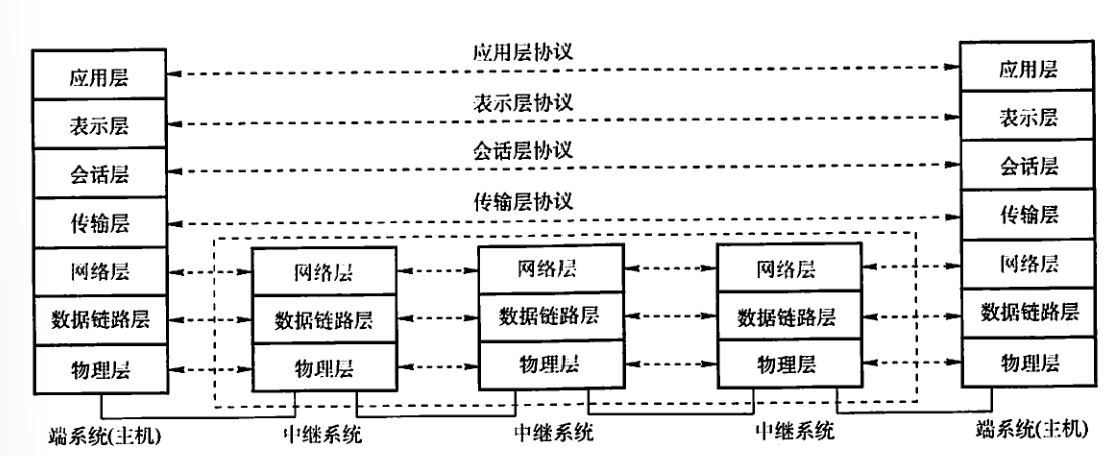
\includegraphics[width=0.8\textwidth]{./images/osi_structure.png}
    \caption{OSI参考模型的层次结构}
\end{figure}
\begin{itemize}
    \item 物理层
    \begin{itemize}
        \item 传输单位:比特
        \item 功能:在物理媒体上为数据端设备透明地传输原始比特流。
        \item 标准:EIA-232C、EIA/TIA RS-449、CCITT的X.21等
        \item 物理媒体本身不属于物理层,可以认为是第零层。
    \end{itemize}
    \item 数据链路层
    \begin{itemize}
        \item 传输单位:帧
        \item 功能:成帧、差错控制、流量控制、传输管理等。
        \item 典型协议:SDLC、HDLC、PPP、STP和帧中继等。
    \end{itemize}
    \item 网络层
    \begin{itemize}
        \item 传输单位:数据报
        \item 功能:路由选择、流量控制、差错控制、拥塞控制、网际互连
        \item 典型协议:IP、IPX、ICMP、IGMP、ARP、RARP、OSPF等
    \end{itemize}
    \item 传输层
    \begin{itemize}
        \item 传输单位:报文段(TCP)或用户数据报(UDP)
        \item 功能:为端到端连接提供可靠的传输服务,是通信子网和资源子网的分界层。
        \item 典型协议:TCP、UDP
    \end{itemize}
    \item 会话层
    \begin{itemize}
        \item 功能:负责在网络中的两节点之间建立、维持和终止通信。
    \end{itemize}
    \item 表示层
    \begin{itemize}
        \item 功能:对上层数据或命令进行解释,以保证一个主机应用层信息可以被另一个主机的应用程序理解。
    \end{itemize}
    \item 应用层
    \begin{itemize}
        \item 典型协议:FTP、SMTP、HTTP等(协议众多)
    \end{itemize}
\end{itemize}

TCP/IP模型和OSI模型的比较:

相同:
\begin{itemize}
    \item 都采用分层的结构
    \item 都基于独立的协议栈的概念
    \item 都可以解决异构网络的互联
\end{itemize}

不同:
\begin{itemize}
    \item OSI精确定义了服务、协议和接口三大概念,TCP/IP则没有明确区分。
    \item OSI是先有模型后有协议,TCP/IP则反之。
    \item OSI是理论上的国际标准,TCP/IP是事实上的国际标准。
    \item (常考)OSI在网络层支持无连接和面向连接的通信,但在传输层仅有面向连接的通信。TCP/IP在网际层仅有一种无连接的通信,但传输层支持无连接和面向连接两种方式。
\end{itemize}

另有一种综合了二者优点的五层结构协议模型,纯粹用于学术研究,没有实际意义。三种模型的比较见图\ref{compare_of_three_architectures}。

\begin{figure}
    \centering
    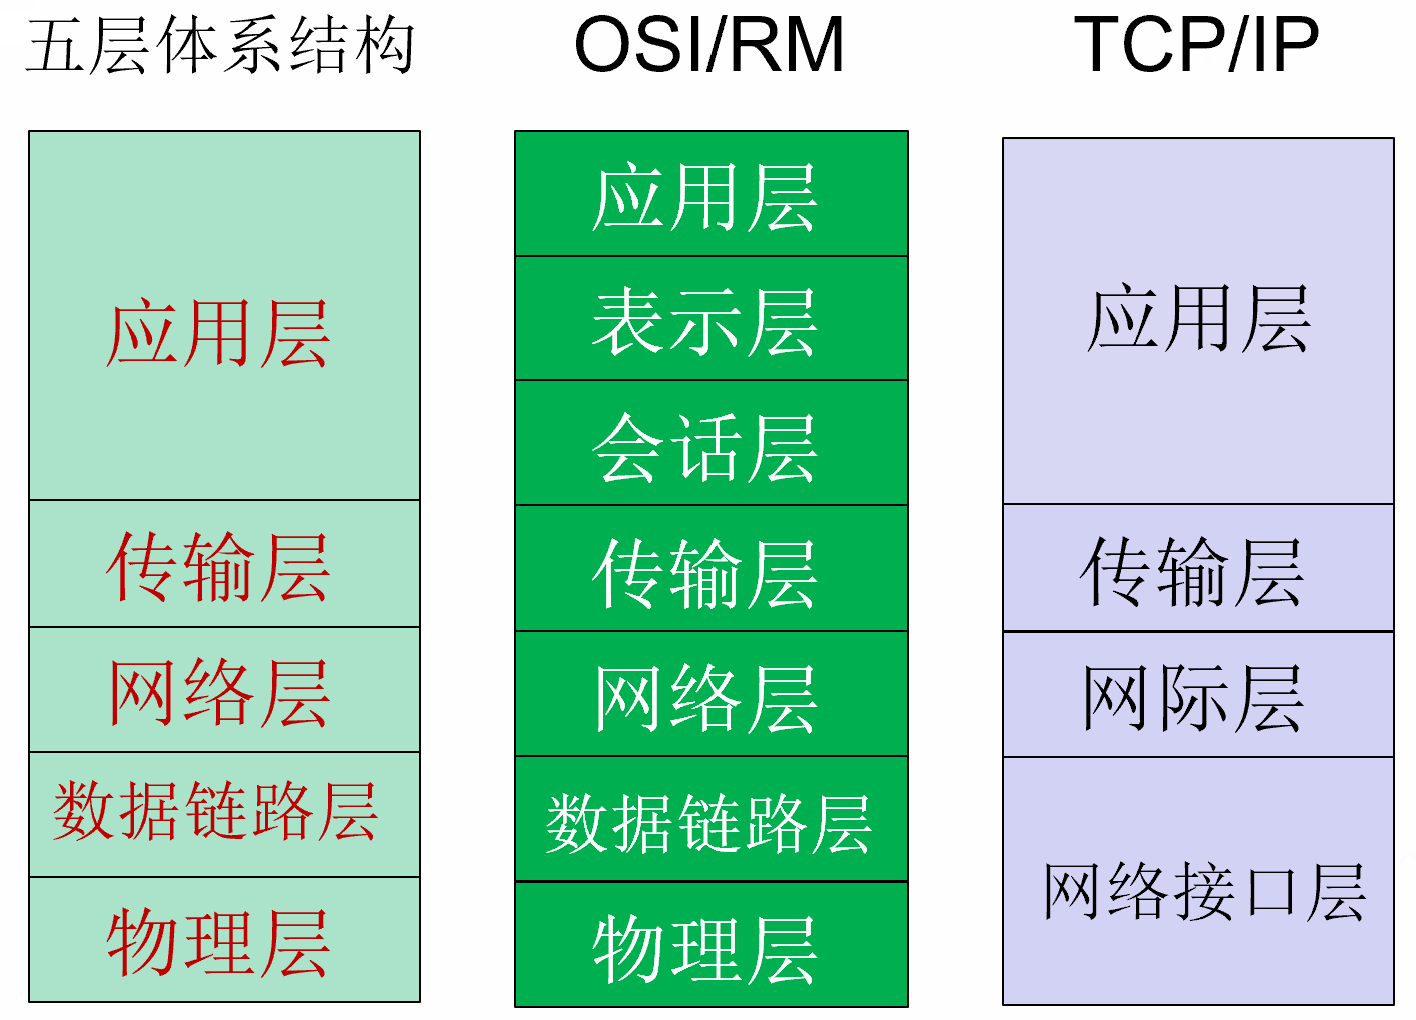
\includegraphics[width=0.6\textwidth]{./images/compare_of_three_architectures.png}
    \caption{三种模型的比较}
    \label{compare_of_three_architectures}
\end{figure}

\section{物理层}

\subsection{通信基础}

通信:将信息从一个地方传送到另外一个地方的过程。

\subsubsection{基本概念}

\begin{enumerate}
    \item 数据、信号与码元
    \begin{itemize}
        \item 数据:传送信息的实体,传输方式可分为串行传输和并行传输,又分:
        \begin{itemize}
            \item 模拟数据:可在某一区间内连续取值的数据。
            \item 数字数据:可在某一区间内取有限个离散值的数据。
        \end{itemize}
        \item 信号:数据的电气或电磁表现。又分:
        \begin{itemize}
            \item 模拟信号:指幅度随时间作连续变化的信号。
            \item 数字信号:指幅度随时间作不连续的、离散变化的信号。
        \end{itemize}
        \item 码元:用一个固定时长的信号波形表示一位$k$进制数字。例如二进制编码时有两种码元,一种代表0,一种代表1。
    \end{itemize}
    \item 信源、信道与信宿
    \begin{itemize}
        \item 这三者是一个数据通信系统的主要组成部分。
        \item 信源是产生和发送数据的源头
        \item 信宿是接收数据的终点
        \item 信道是传输信号的通路。
    \end{itemize}
    \begin{figure}[h]
        \centering
        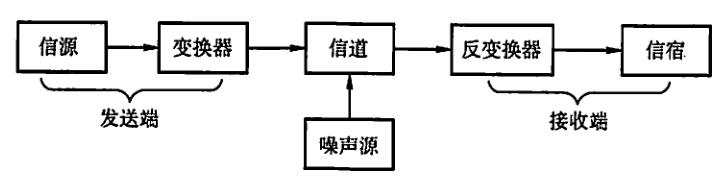
\includegraphics[scale=1]{./images/single_communication_system.png}
        % \begin{tikzpicture}[node distance=50pt]
        %     \node[draw, rounded corners] (source) {信源};
        %     \node[draw, rounded corners, right of=source] (transformer) {变换器};
        %     \node[draw, rounded corners, right of=transformer] (channel) {信道};
        %     \node[draw, rounded corners, right of=channel] (intransformer) {反变换器};
        %     \node[draw, rounded corners, right of=intransformer] (destination) {信宿};
        %     \node[draw, rounded corners, below of=channel] (noise) {噪声源};
        %     \draw[->] (source) -- (transformer);
        %     \draw[->] (transformer) -- (channel);
        %     \draw[->] (channel) -- (intransformer);
        %     \draw[->] (intransformer) -- (destination);
        %     \draw[->] (noise) -- (channel);
        % \end{tikzpicture}
        \caption{单向通信系统模型}
    \end{figure}
    \item 速率、波特与带宽
    \begin{itemize}
        \item 速率指的是数据传输速率,可以用如下两种方式表示:
        \begin{itemize}
            \item 码元传输速率(波特率):表示通信系统传输码元的速率,单位是波特(1波特表示每秒传输一个码元),与传输的进制无关。
            \item 信息传输速率(比特率):表示通信系统传输\textbf{二进制}码元的速率,单位是比特/秒。
            \item 若一个码元携带$n$比特的信息量,则$M$波特率的码元传输速率对应的信息传输速率为$Mn$比特/秒。
        \end{itemize}
        \item 带宽:见\ref{performance_index}节。
    \end{itemize}
\end{enumerate}

\textbf{数据传输方式}
\begin{itemize}
    \item 从通信双方信息的交互方式看,可分为\textbf{三种}基本方式:
    \begin{itemize}
        \item 单向通信:如无线电广播、电视广播
        \item 半双工通信:可以双向发送信息,但任何一方都不能同时发送和接收信息。
        \item 全双工通信:通信双方可以同时发送和接收信息。
    \end{itemize}
    \item 从双方是否同步来看,可分为:
    \begin{itemize}
        \item 同步方式
        \item 异步方式
    \end{itemize}
    \item 从串并行来看,可分为:
    \begin{itemize}
        \item 串行方式
        \item 并行方式
    \end{itemize}
\end{itemize}

\subsubsection{奈奎斯特定理}

码间串扰现象:信道通过高频分量的效果往往较差,从而导致接收端接收到的信号波形失去码元之间的清晰界限。

奈奎斯特(Nyquist)定理指出:在理想低通(无噪声,带宽有限)的信道中,为了避免码间串扰,极限码元传输速率为$2W$波特,其中$W$是理想低通信道的带宽。

根据奈奎斯特定理,可以得出如下结论:
\begin{enumerate}
    \item 在任何信道中,码元传输速率是有上限的。若超过此上限,就会出现严重的码间串扰问题。
    \item 频道的频带越宽,传输码元的极限速率就越高。
\end{enumerate}

\subsubsection{香农定理}

香农定理给出了带宽受限且有高斯白噪声干扰的信道的极限数据传输速率:
\begin{equation*}
    \text{极限速率}C=W\text{log}_2(1+\frac{S}{N})
\end{equation*}
其中
\begin{itemize}
    \item $W$为信道带宽
    \item $S$为信道传输信号的平均功率
    \item $N$为信号内部的高斯噪声功率
\end{itemize}

根据香农定理,可以得出如下结论:
\begin{enumerate}
    \item 信道的带宽或信道中的信噪比($S/N$)越大,信息的极限传输速率$C$就越高。$N\to 0$时,$C\to\infty$,因此无干扰信道容量为无穷大。
    \item 对于一定的带宽和一定的信噪比,信息传送速率的上限是确定的。
    \item 只要信息传输速率低于信道的极限速率,就能找到某种办法实现无差错的传输。
    \item 设$N_0$为频谱密度,则有$N=N_0\times B$。当$W\to \infty$时,$C\to 1.44\frac{S}{N_0}$,并不会趋于无穷大。
\end{enumerate}

\subsubsection{编码}

\begin{enumerate}
    \item {\bf 归零编码}。每个时钟周期的中间都要归零,提供了自同步机制,但归零要占用一点带宽。
    \item {\bf 非归零编码}。不归零,但无法同步,需要额外的时钟线。
    \item {\bf 反向非归零编码}。用信号的反转代表0,信号保持不变代表1,有同步且不会占用带宽。
    \item {\bf 曼彻斯特编码}。将一个码元分成两个相等的间隔。实际上有两种截然相反的约定,较常用的一种是:前高后低为0,1则相反。也可同步。
    \begin{itemize}
        \item 用于802.3局域网(以太网)。
    \end{itemize}
    \item {\bf 差分曼彻斯特编码}:若电平和上一个码元结束的电平一致,表示1,否则表示0。每个码元中间有一次跳变,用于同步。
    \begin{itemize}
        \item 用于802.5局域网(令牌环网)。
    \end{itemize}
\end{enumerate}

\subsubsection{调制}

\begin{enumerate}
    \item 数字信号转模拟信号
    \begin{itemize}
        \item 幅移键控(ASK),又称调幅
        \item 频移键控(FSK),又称调频
        \item 相移键控(PSK),又称调相
        \item 正交振幅调制(QAM)
    \end{itemize}
    \item 模拟信号转数字信号
    \begin{itemize}
        \item 采样
        \item 量化
        \item 编码
    \end{itemize}
\end{enumerate}

\subsubsection{电路交换、报文交换与分组交换}

\begin{enumerate}
    \item {\bf 电路交换}
    
    进行数据传输前,两个节点之间建立一条双方独占的物理通信路径。这条路径一直被独占到连接释放为止。

    优点:
    \begin{itemize}
        \item 通信时延小。
        \item 有序传输。
        \item 没有冲突。
        \item 适用范围广,适用于模拟信号和数字信号。
        \item 实时性强。
        \item 控制简单。
    \end{itemize}
    缺点:
    \begin{itemize}
        \item 建立连接时间长。
        \item 线路独占,效率低。
        \item 灵活性差。
        \item 难以规格化。
    \end{itemize}
    \item {\bf 报文交换}
    
    优点:
    \begin{itemize}
        \item 无须建立连接。
        \item 动态分配线路。
        \item 线路可靠性高。如果一条路径故障,还可以选择另一条路径。
        \item 线路利用率高。
        \item 可以提供多目标服务。
    \end{itemize}
    缺点:
    \begin{itemize}
        \item 由于每个节点都要存储-转发,因此会有转发时延。
        \item 要求节点有较大的缓存空间。
    \end{itemize}
    报文交换多用于早期的电报通信网络中,现已很少用。现在常用的是分组交换。
    \item {\bf 分组交换}
    
    优点:
    \begin{itemize}
        \item 无建立时延。
        \item 线路利用率高。
        \item 相对于报文交换,简化了存储管理。
        \item 加速传输。分组的传输可以并行化。
        \item 减少了出错概率和重发数据量。因分组较短,故出错概率必然减小。
    \end{itemize}
    缺点:
    \begin{itemize}
        \item 存在传输时延。
        \item 需要处理额外的信息量。
        \item 分组可能失序、丢失或者重复,需要在接收端重排检错。
    \end{itemize}
    分组交换比报文交换的时延小,尤其适合于计算机系统的猝发式通信。
\end{enumerate}

\subsubsection{数据报与虚电路}

它们都属于网络层,都是分组交换的方式。

\begin{figure}
    \centering
    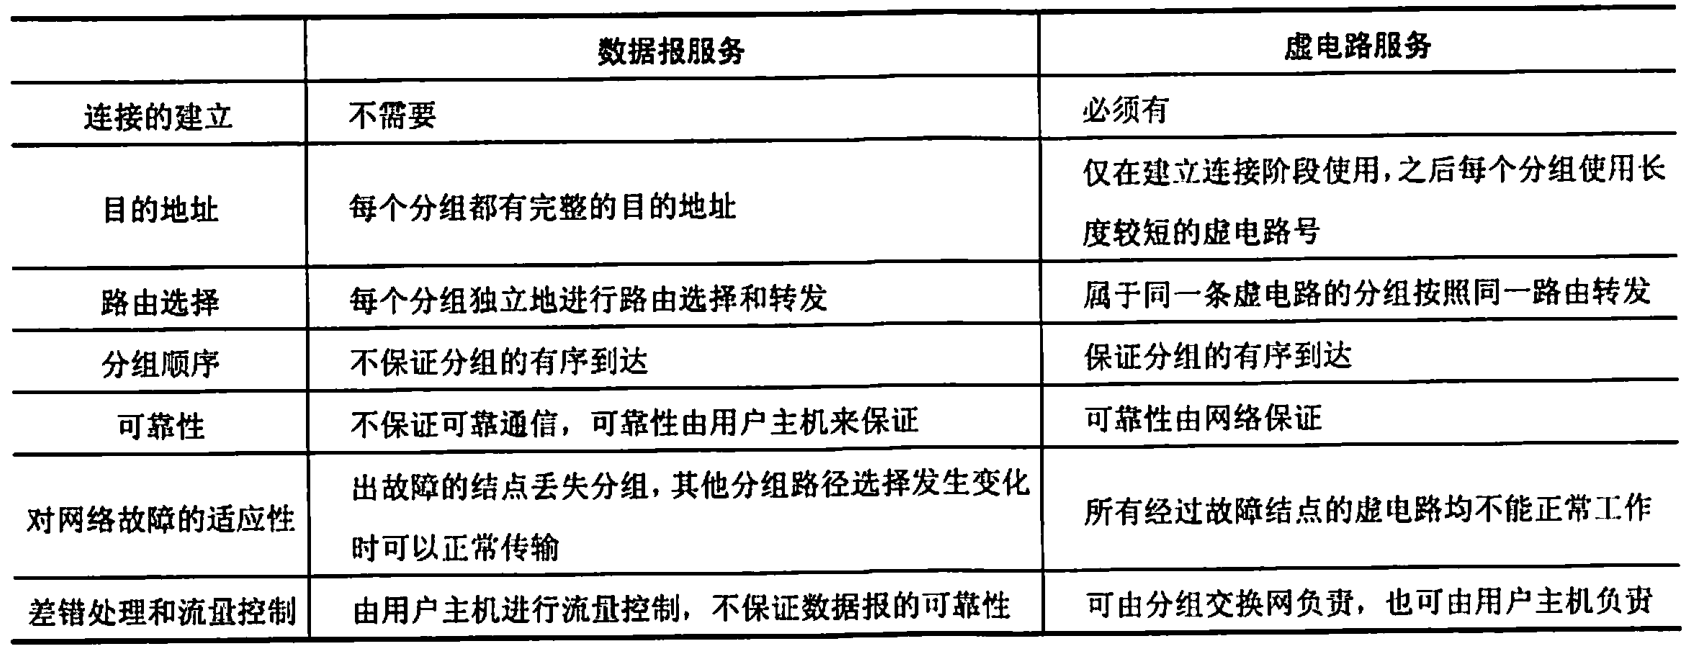
\includegraphics[width=\textwidth]{./images/datagram_and_virtual_circuit.png}
    \caption{数据报和虚电路的比较}
\end{figure}

\subsection{传输介质}

\subsubsection{双绞线、同轴电缆、光纤与无线传输介质}

\begin{enumerate}
    \item {\bf 双绞线}
    
    最常用的古老传输介质,由两根并排绞合、相互绝缘的铜线构成。价格便宜,在局域网和电话网络中普遍使用。
    \item {\bf 同轴电缆}
    
    抗干扰性能良好,传输距离远,价格稍贵。
    \item {\bf 光纤}
    
    带宽范围极大,传输损耗小,抗大电流脉冲干扰(如雷电),保密性佳,体积小,重量轻。
    \item {\bf 无线传输介质}
\end{enumerate}

\subsubsection{物理层接口的特性}

\begin{itemize}
    \item 机械特性
    \item 电气特性
    \item 功能特性
    \item 过程特性
\end{itemize}

\subsection{物理层设备}

\subsubsection{中继器}

主要作用是将信号整形并放大再转发出去,以消除信号的失真和衰减。

中继器放大数字信号,另有一种放大模拟信号的设备是放大器。

\subsubsection{集线器}

集线器(Hub)实际上是一个多端口的中继器。集线器在收到数据信号后,进行整形放大,然后转发到其他所有端口(不含输入端口)。

集线器只能在半双工条件下工作。

\section{数据链路层}

\textbf{数据链路层三大基本问题:}
\begin{itemize}
    \item {\bf 封装成帧}:为了实现传输中的检错纠错,以及部分重发功能,必须将物理层的比特流封装成帧来发送。实现方法是在帧的开始和结束位置插入帧定界符。
    \item {\bf 透明传输}:这是指无论被传数据是什么样的比特组合,都能够在链路上传送。解决办法是使用字节填充法或比特填充法。
    \item {\bf 差错控制}:这里的差错控制主要针对冲击噪声。解决办法是通过特殊的编码(差错控制码),使接收端能够发现甚至自动纠正错误。
\end{itemize}

\subsection{数据链路层的功能}

主要作用:加强物理层传输原始比特流的功能,将物理层提供的可能出错的物理连接改造为逻辑上无差错的数据链路。

\subsubsection{为网络层提供服务}

数据链路层通常可为网络层提供如下服务:
\begin{enumerate}
    \item 无确认的无连接服务:无需预先建立连接,目的机器收到数据帧后无需确认。如以太网。
    \item 有确认的无连接服务。如无线通信。
    \item 有确认的面向连接服务。
\end{enumerate}

\subsubsection{链路管理}

指的是数据链路层连接的建立、维持和释放过程。

\subsubsection{帧定界、帧同步与透明传输}

将网络层数据的前后分别添加首部和尾部,就构成了帧。

透明传输问题:不管所传数据是什么样的比特组合,都应当能在链路上传送。

\subsubsection{流量控制}

实际上是限制发送方的数据流量,使之不超过接收方的能力限制。

运输层也有流量控制机制,但数据链路层的流量控制是控制相邻两个节点之间的流量,而传输层控制的是源端到目的端之间的流量。

\subsubsection{差错控制}

数据链路层中的错误可以分成位错和帧错两种。
\begin{itemize}
    \item {\bf 位错}。指帧当中的某些位出现了差错,通常采用循环冗余校验(CRC)方法发现错误,通过自动重传请求(ARQ)方法重传。接收方检测到错误之后直接丢弃帧,发送方计时超时后就自动重传。
    \item {\bf 帧错}。指帧的丢失、重复、失序等错误。数据链路层引入定时器和编号机制,确保此类错误被正确解决。
\end{itemize}

差错出现的原因可以是热噪声或冲击噪声,差错控制机制主要处理冲击噪声造成的差错。

\subsection{组帧}

\subsubsection{字符计数法}

指的是在帧头部使用一个计数字段来标明帧内的字符数。最大的问题是一旦这个字段出错,那么双方就立即失去同步,后面的所有帧都要废弃。

\subsubsection{字符填充的首尾定界符法}

指的是使用特殊的字符来标志一帧的开始和结束。

\subsubsection{零比特填充的首尾标志法}

使用一个特定的比特模式即01111110(0+6个1+0)来标志一帧的开始和结束。发送方在正式的数据中如果遇到连续5个1,就在后面插入一个0,这样不致和首尾标志混淆。接收方遇到连续5个1后,检查后面的位,如果是1,表示是首尾标志;如果是0,表示是数据,将删去这个0。

\subsubsection{违规编码法/违例编码法}

一些编码中的某些模式是“违规”的,即正常情况下一定不会出现,可以利用这种违规序列来标志首尾。局域网的IEEE802标准就用了此法。

目前最常用的后两者。

\subsection{差错控制}

\subsubsection{检错编码}

检错编码都采用冗余编码技术。常见的检错编码有奇偶校验码和循环冗余(CRC)码。

CRC码有纠错功能,但数据链路层只使用了它的检错功能。

编码效率$R$:码字中信息位所占的比例。若码字中信息位为$k$位,编码时外加的冗余位为$r$位,则编码后的码字长为$n=k+r$位,这时有
\begin{equation*}
    R=\frac{k}{n}=\frac{k}{k+r}
\end{equation*}

\begin{enumerate}
    \item {\bf 奇偶校验码}
    
    是通过增加冗余位来使得码字中1的个数保持奇数或偶数的编码方法。通信中又可分为:
    \begin{itemize}
        \item 垂直奇偶校验
        \item 水平奇偶校验
        \item 水平垂直奇偶校验
    \end{itemize}

    \item {\bf 循环冗余(CRC)码}
    
    模2运算:不看进位和借位,加减就是异或。

    模2除的上商原则(重要):
    \begin{itemize}
        \item 部分余数的首位为1时,上1
        \item 部分余数的首位为0时,上0
        \item 部分余数的位数少于除数的位数时,停止除法,该部分余数就是最后的余数。
        \item 也就是说,上商只无脑看首位数字,不比较大小。
    \end{itemize}
    
    引入一种多项式记法,这种多项式和一个二进制位序列是一一对应的。比如,1101对应的多项式$M(x)$为:
    \begin{equation*}
        M(x)=1\cdot x^3+1\cdot x^2+0\cdot x^1+1\cdot x^0
    \end{equation*}

    现有待计算的信息位串$M(x)$,又有固定的生成多项式$G(x)$,则计算CRC码的过程如下:
    \begin{enumerate}
        \item 令$r=G(x)\text{位数}-1$,如$G(x)=1011$,4位,则$r=3$。
        \item 将$M(x)$左移$r$位。右边补零。
        \item 用模2除的方法计算
        \begin{equation*}
            \frac{M(x)\cdot x^r}{G(x)}
        \end{equation*}
        得到余数,把这余数加到左移后的$M(x)$,就得到CRC编码。
    \end{enumerate}

    接收到CRC码$T(x)$后,将$T(x)$与同一生成多项式$G(x)$作模2除运算,如果余数为0,表示无误,否则表示出现错误。
\end{enumerate}

\begin{problem}
    信息位串为1010001,生成多项式$G(x)=x^4+x^2+x+1$,求CRC码。 
\end{problem}
\begin{solution}
    \begin{enumerate}
        \item $M(x)=x^6+x^4+1$,由$G(x)$得$r=4$。
        \item $M(x)$左移4位,得到10100010000。
        \item 计算$\frac{M(x)\cdot x^r}{G(x)}$的余数,结果为1101,过程见图\ref{crc_example}。
        \item 将1101加到左移后的$M(x)$,得到CRC码10100011101。
    \end{enumerate}
\end{solution}

\begin{figure}[h]
    \centering
    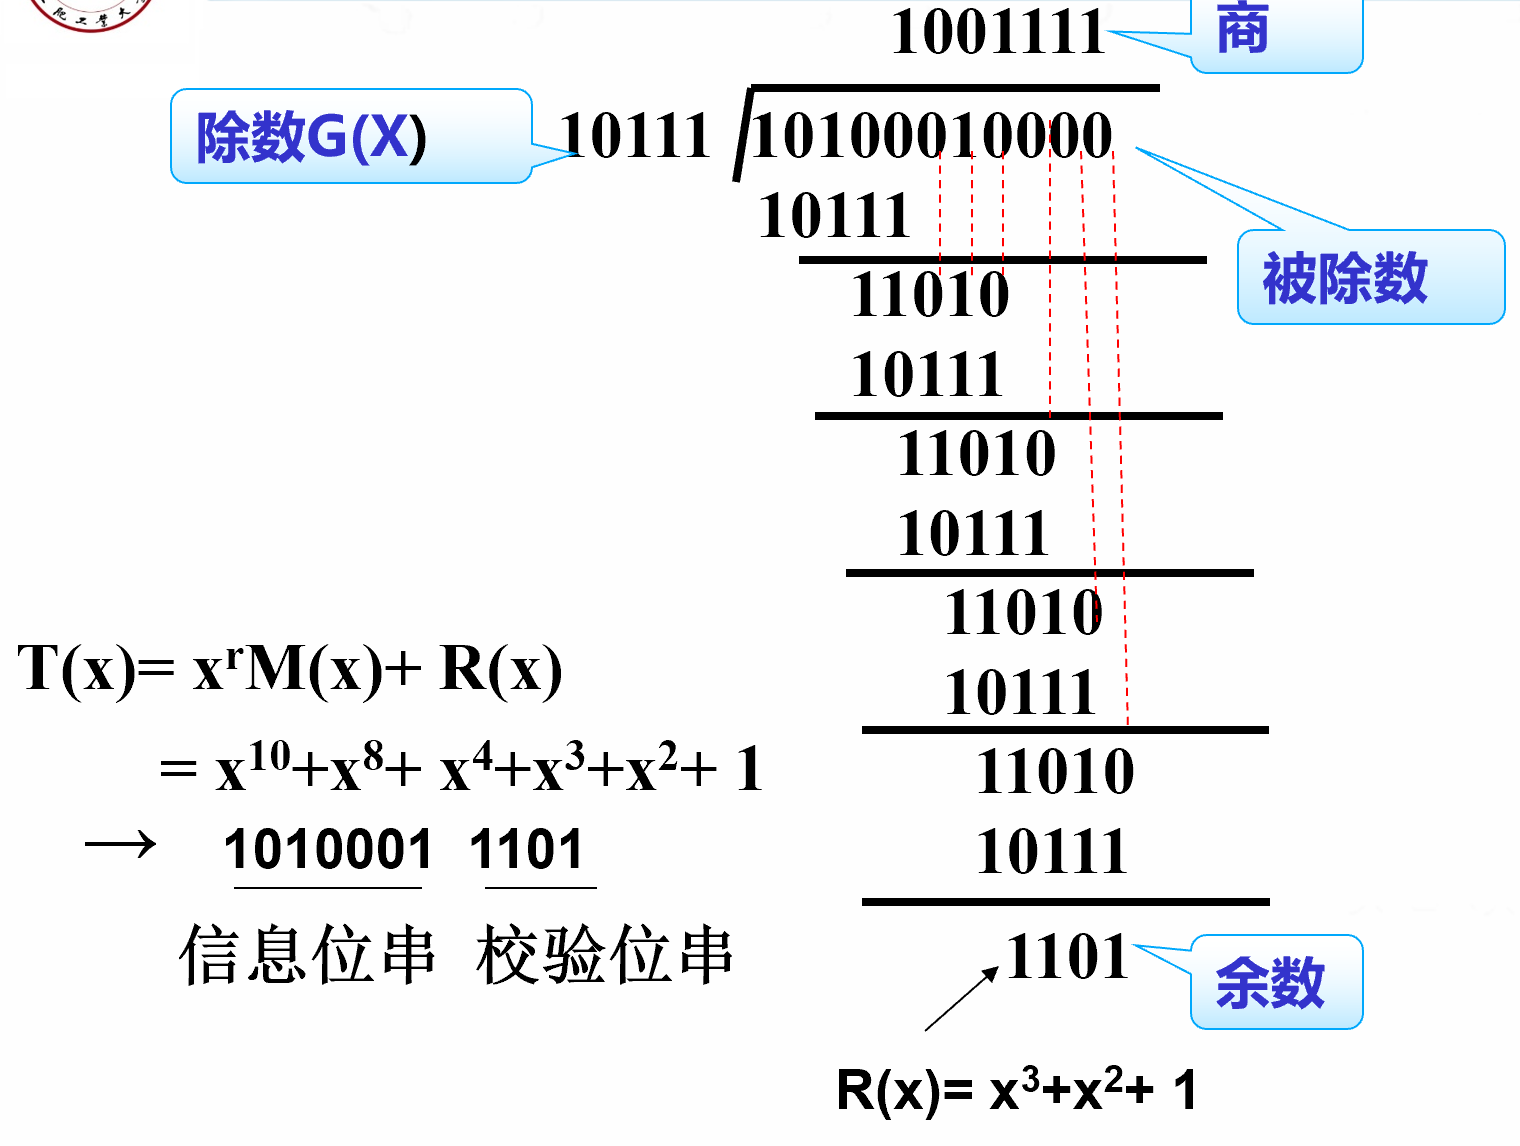
\includegraphics[width=0.6\textwidth]{./images/crc_encode_example.png}
    \caption{模2除的计算过程}
    \label{crc_example}
\end{figure}

\subsubsection{纠错编码}

最常见的纠错编码是海明码。

\subsection{流量控制与可靠传输机制}

\subsubsection{流量控制、可靠传输与滑动窗口机制}

流量控制的基本方法是由接收方控制发送方发送数据的速率。常见的方式是停止-等待协议和滑动窗口协议。
\begin{itemize}
    \item 停止-等待协议:发送方每发送一帧,就必须等待接收方的应答信号,才能发送下一帧。效率很低。
    \item 滑动窗口协议:发送端每收到一个帧的确认,发送窗口就向前滑动一个帧的位置;接收端收到数据帧后,将接收窗口向前移动一个位置,并发回确认帧。若收到的数据帧落在窗口之外,则一律丢弃。
\end{itemize}

数据链路层的滑动窗口协议中,窗口大小是固定的,这一点与TCP不同。

如果滑动窗口的大小为1,可保证帧的有序接收。

传统的自动重传请求(ARQ)可分为三种:
\begin{itemize}
    \item 停止-等待ARQ
    \item 后退N帧ARQ
    \item 选择性重传ARQ
\end{itemize}

\subsubsection{单帧滑动窗口与停止-等待协议}

\subsubsection{多帧滑动窗口与后退N帧协议(GBN)}

在后退N帧ARQ中,发送方可以连续发送帧,不需要等待确认。如果接收方检测出失序的帧,就要求发送方重发第一个出错帧(含)之后的所有帧。也就是说,接收方只允许顺序接收帧,对某个帧的确认就表明该帧之前的所有帧都已正确无误地收到。

若信道的误码率较大,后退N帧ARQ未必就比停止-等待ARQ好。

\subsubsection{多帧滑动窗口与选择重传协议(SR)}

\subsection{介质访问控制}

介质访问控制的任务是,为使用介质的每个节点隔离来自同一信道上的其他节点所传送的信号。即采取一定的措施,使得两对节点之间的通信不会发生互相干扰的情况。

常见的介质访问控制方法包括:
\begin{itemize}
    \item 信道划分介质访问控制(静态划分信道)
    \item 随机访问介质访问控制(动态分配信道)
    \item 轮询访问介质访问控制(动态分配信道)
\end{itemize}

\subsubsection{信道划分介质访问控制}

信道划分的实质是:通过分时、分频、分码等方式把原来的一条广播信道,逻辑上分为几条用于两个节点之间通信的互不干扰的子信道。实际上是把广播信道转变为点对点信道。

信道划分介质访问控制可以分为以下4种:
\begin{enumerate}
    \item {\bf 频分多路复用(FDM)}
    
    是指将多路基带信号调制到不同的频率载波上,叠加形成一个复合信道的多路复用技术。为了避免不同子信道的干扰,需要在相邻信道之间加入“保护频带”。

    优点是技术成熟,实现容易,系统效率高。
    \item {\bf 时分多路复用(TDM)}
    
    是指将一条物理信道按时间分成若干时间片,轮流地分给多个信号使用,每个时间片由当前的信号独占。

    传统TDM是机械地按照信号数量平均分配时间片,而改进的\textbf{统计时分多路复用(STDM)}允许按照需要动态分配时间片,某个信号在其他信号都发送数据时,有可能独占全部时间。
    \item {\bf 波分多路复用(WDM)}
    
    这实际上是光纤条件下的概念,是指光的频分多路复用。由于光的波长(频率)不同,各路光信号之间互不干扰。
    \item {\bf 码分多路复用(CDM)}
    
    指的是采用不同的编码来区分各路原始信号的多路复用方式。CDM同时共享了时间和频率。

    实际上更常用的术语是码分多址(CDMA)。

    CDM频谱利用率高、抗干扰能力强、保密性好,还可以降低成本,多用于无线通信系统。
\end{enumerate}

\subsubsection{随机访问介质访问控制}

随机访问介质访问控制中,不采用中心化的控制方式,而是所有用户根据自己的意愿随意发送信息,但发生冲突时必须重传冲突的帧,直到帧被正确接收。重传的规则称为随机访问介质访问控制协议。常用的协议有:
\begin{enumerate}
    \item {\bf ALOHA协议}
    
    又可分为纯ALOHA和时隙ALOHA两种。
    \begin{enumerate}
        \item {\bf 纯ALOHA协议}
        
        站点可以不经过任何检测就发送数据。如果一段时间内没有收到确认,就等待一段随机时间后重发,直至发送成功。吞吐量很低。
        \item {\bf 时隙ALOHA协议}
        
        让所有站点在时间上同步,并把时间划分成若干等长的时隙(Slot),规定只能在每个时隙开始时发送一个帧。处理冲突的策略和纯ALOHA一样。
    \end{enumerate}
    \item {\bf CSMA协议}
    
    载波侦听多址访问(CSMA)协议和ALOHA的区别是多了一个载波侦听装置,发送前需要先侦听信道是否空闲。

    根据侦听方式和侦听到信道忙之后的处理方式不同,CSMA协议可分为三种。
    \begin{enumerate}
        \item {\bf 1-坚持CSMA}
        
        首先侦听信道,如果信道空闲,就立即发送数据;如果信道忙,就持续侦听直至信道空闲,然后立即发送数据。如果遇到冲突,那么等待随机一段时间后再侦听信道。

        “1-坚持”的含义是:侦听到信道忙后,继续坚持侦听信道;侦听到信道空闲后,发送帧的概率为1,即立即发送数据。
        \item {\bf 非坚持CSMA}
        
        和1-坚持CSMA的不同是,如果信道忙,就放弃侦听,等待一段随机时间后再侦听信道。

        非坚持CSMA降低了冲突发生的概率,但是会增加网络的延迟。
        \item {\bf $p$-坚持CSMA}
        
        首先侦听信道,如果信道忙,就持续侦听到信道空闲,;如果信道空闲,就以概率$p$发送数据,以概率$1-p$推迟到下一个时隙,下一个时隙依然如此,直到成功发送数据或者侦听到信道忙为止。

        \begin{table}[h]
            \centering
            \resizebox{\linewidth}{!}{
                \begin{tabular}{c|c|c|c}
                    \hline
                    信道状态 & 1-坚持 & 非坚持 & $p$-坚持 \\
                    \hline
                    空闲 & 立即发送数据 & 立即发送数据 & 以概率$p$发送数据,以概率$1-p$推迟到下一个时隙 \\
                    \hline
                    忙 & 继续侦听 & 放弃,等待一个随机事件后再侦听 & 持续侦听,直至信道空闲 \\
                    \hline
                \end{tabular}
            }
            \caption{三种不同类型的CSMA协议的比较}
        \end{table}
    \end{enumerate}

    \item {\bf CSMA/CD协议}
    
    这是CSMA的改进版本,用于有线连接的局域网,如总线形网络或半双工网络环境。发送数据前先侦听总线上有无其他站点正在发送数据,如有则等待至空闲,若无则发送数据,但同时要持续监听总线上有无其他信号。若检测到冲突,就发送一个拥塞信号(jamming signal),让其他所有站点都知道。中止发送后,执行指数避退算法。

    注意:监听时发现信道空闲,不意味着信道就真的是空闲的,可能其他站点也在发送数据,但数据还在传播过程中。

    设端到端传播时延为$\tau$,则某个站发送帧之后至多经过$2\tau$就可以得知是否发生碰撞。因此把这个$2\tau$称为\text{争用期}(或冲突窗口、碰撞窗口)。

    CSMA/CD要求一个帧的传输时延必须大于$2\tau$,否则一个帧发送完毕后就无法再跟踪它是否出现冲突了。凡小于$2\tau$的帧都是无效帧,应该直接丢弃。如果一个帧确实没有$2\tau$长,就应该在后面加入填充字段。

    \textbf{二进制指数避退算法}
    \begin{itemize}
        \item 确定基本避退时间,一般取$2\tau$。
        \item 定义参数$k$,其中$k=\text{min}[\text{重传次数}, 10]$。
        \item 从整数集合$[0,1,\cdots,2^k-1]$中随机取出一个数$r$,重传的避退时间就是$2\tau r$。
        \item 重传16次后仍然不成功时,放弃重传,并向高层报告错误。
    \end{itemize}
    \item {\bf CSMA/CA协议}
    
    适用于无线连接的局域网。与CSMA/CD的不同是,CSMA/CA要尽量避免碰撞的发生。
\end{enumerate}

\subsubsection{轮询访问:令牌传递协议}

\subsection{局域网}

\subsection{广域网}

\subsection{数据链路层设备}

\section{网络层}

\subsection{网络层的功能}

\subsubsection{异构网络互联}

中继系统分为以下4种:
\begin{itemize}
    \item 物理层:转发器、集线器
    \item 数据链路层:网桥、交换机
    \item 网络层:路由器
    \item 网络层以上:网关
\end{itemize}

前两层只是把网络扩大了,从网络层的角度看,并不能算是网络互联。

\begin{itemize}
    \item 路由器不转发广播包,因此能够分隔广播域,抑制网络风暴。
    \item 交换机可以分隔冲突域,但不能分隔广播域。
    \item 集线器和中继器既不能分隔冲突域又不能分隔广播域。
\end{itemize}

使用IP网络的好处:屏蔽互联的各网络的异构细节(如编址方案、路由选择协议等)。

\begin{problem}
    在路由器互联的多个局域网的结构中,要求每个局域网(\ \ )
\end{problem}
\begin{solution}
    物理层、数据链路层、网络层协议可以不同,高层协议必须相同
\end{solution}
\begin{note}
    网络层协议不同而实现互联的例子:使用特定的路由器连接IPv4和IPv6网络
\end{note}

\subsubsection{路由与转发}

路由器的两大任务:
\begin{itemize}
    \item 路由选择
    \item 分组转发
\end{itemize}

路由表是由路由选择算法得出的,转发表是从路由表得出的。

\subsubsection{SDN的基本概念}

待补

\subsubsection{拥塞控制}

在通信子网中,因出现过量的分组而引起网络性能下降的现象称为\textbf{拥塞}。

通过观测网络吞吐量随网络负载的变化关系,可以估计网络的拥塞程度。

拥塞控制的方法:
\begin{itemize}
    \item {\bf 开环控制}。静态的方法,在设计网络时考虑各种因素,一旦确定就不再更改。
    \item {\bf 闭环控制}。动态的方法,监视网络的状态,检测哪里发生了拥塞,并调整网络。
\end{itemize}

拥塞控制和流量控制的区别:
\begin{itemize}
    \item 流量控制指的是发送端和接收端之间的点对点通信量的控制。
    \item 拥塞控制是全局性问题,涉及整个网络的所有主机、路由器。
\end{itemize}

\subsection{路由算法}

\subsubsection{静态路由与动态路由}

\begin{itemize}
    \item 静态路由算法(非自适应路由算法):需要网络管理员手动配置路由信息,不能及时适应网络状态的变化。适用于小型网络。
    \item 动态路由算法(自适应路由算法):可以动态适应网络状态。又分:
    \begin{itemize}
        \item 距离向量路由算法(D-V):典例是RIP算法
        \item 链路状态路由算法(L-S):典例是OSPF算法
    \end{itemize}
\end{itemize}

\subsubsection{距离向量路由算法}

所有的节点都定期地将它们的整个路由表发给\textbf{相邻}的节点。这表包含:
\begin{itemize}
    \item 每条路径的目的地(另一节点)
    \item 路径的代价(距离)
\end{itemize}

D-V协议中,好消息传得快,坏消息传得慢。当路由信息发生变化时,旧的信息可能还在网络中传递。这就是“慢收敛”。慢收敛是导致路由环路的根本原因。

可以想见,网络规模越大,交换的信息也越多。因此这种算法不适合大规模网络。

\subsubsection{链路状态路由算法}

定期将自己与\textbf{相邻节点}的链路状态(如距离、时延、带宽、费用等)向全网\textbf{所有节点}泛洪。之后各节点通过Dijkstra算法生成路由表。

L-S算法发送的数据链不会随着网络规模的增大而增长,因而适合大规模网络。

\subsubsection{层次路由}

Internet将整个互联网划分为许多较小的自治系统。每个自治系统有权决定系统内部使用何种路由选择协议。
\begin{itemize}
    \item 一个自治系统内部使用的路由选择协议称为\textbf{内部网关协议(IGP)},具体包括RIP和OSPF等。
    \item 自治系统之间使用的路由选择协议称为\textbf{外部网关协议(EGP)},如BGP协议。
\end{itemize}

\subsection{IPv4}

IP需要ICMP、ARP、RARP等路由协议的支持。

\subsubsection{IPv4分组}

IP分组=首部+数据。

首部=固定字段(20B长)+可选字段

\begin{figure}
    \centering
    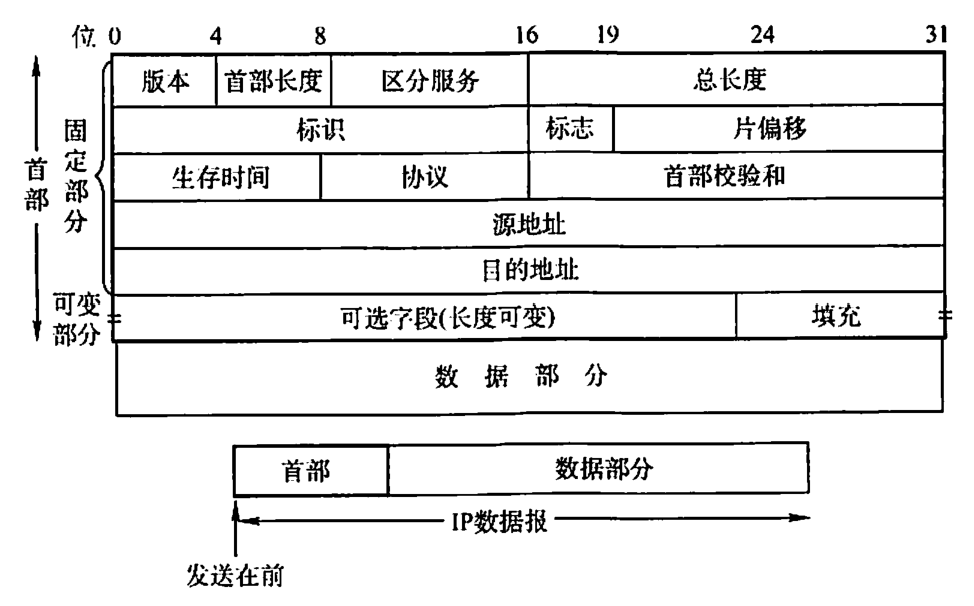
\includegraphics[width=0.8\textwidth]{./images/ip_datagram.png}
    \caption{IP数据报的格式}
\end{figure}

\begin{enumerate}
    \item {\bf 版本}。指IP协议的版本,可以是4或者6。
    \item {\bf 首部长度}。最大值是60B,最常用的是20B(无扩展)
    \item {\bf 区分服务},用来指明要求网络提供的服务,实际上从未使用过。
    \item {\bf 总长度},指整个IP分组的长度。最长为65536B。
    \item {\bf 标识},用来标识数据报的顺序。如果数据报产生了分片,那么所有分片将共用同一个标识。
    \item {\bf 标志},占3位,第二位是MF,第三位是DF,第一位(最高位)保留。
    \item {\bf 片偏移},如果产生分片,则本字段指出当前分片相对于数据报头的偏移量。单位是8B,所以除最后一个分片外,所有分片长度都是8B的整数倍。
    \item {\bf 生存时间TTL},标识分组的寿命。路由器转发分组前先把TTL减一。若TTL减至0则丢弃。
    \item {\bf 协议},指分组携带的数据使用的传输层协议。值6表示TCP,17表示UDP。
    \item {\bf 首部校验和},只校验首部,不校验数据部分。
    \item {\bf 源地址},标识发送方的IP地址。
    \item {\bf 目的地址},标识接收方的IP地址。
\end{enumerate}

首部长度、总长度、片偏移是IP分组中有关长度的3个字段。它们的基本单位分别是4B、1B和8B(常考加减)。

一个链路层数据报能承载的最大数据量称为最大传送单元(MTU)

对标志字段的进一步解释:
\begin{itemize}
    \item DF(Don't Fragment)表示数据报是否允许分片,1不允许,0允许。
    \item MF(More Fragment)表示后面还有没有更多的分片。1表示还有,0表示没有(即当前分片是最后一个分片)。
\end{itemize}

\subsubsection{IPv4地址与NAT}

图\ref{ip_classes}示出了传统分类IP地址的分类情况。

\begin{figure}[h]
    \centering
    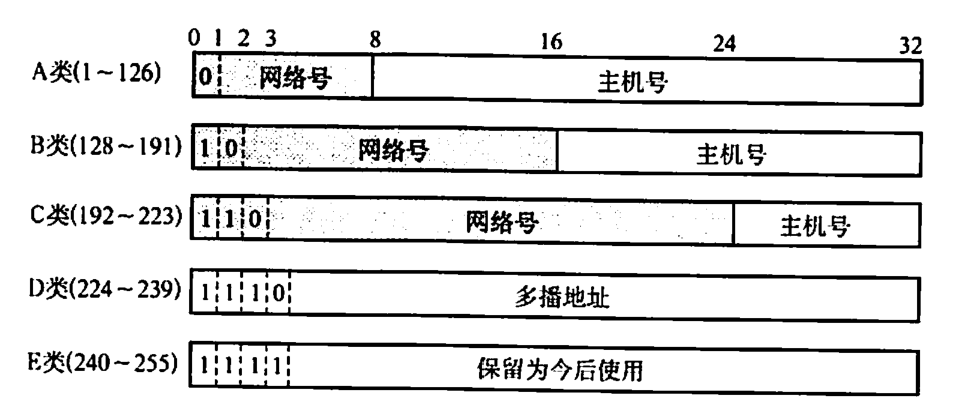
\includegraphics[width=0.8\textwidth]{./images/ip_address.png}
    \caption{分类的IP地址}
    \label{ip_classes}
\end{figure}

IP地址::=\{<网络号>,<主机号>\}

特殊的IP地址:
\begin{itemize}
    \item 主机号全0表示主机所在的网络本身。
    \item 主机号全1表示主机所在的网络的广播地址。
    \item 127.*.*.*保留为环回自检地址。
    \item 0.0.0.0表示本机。系统启动时用到,启动后不再使用。
    \item 255.255.255.255表示整个网络的广播地址,实际上是本网络的广播地址。
\end{itemize}

网络地址转换(NAT)技术将专用地址转换为公用地址,从而大大节省了IP地址的消耗。

本地主机与外部网络通信时,NAT路由器通过NAT转换表完成本地IP和全球IP的转换。转换表的项都是\{本地IP:端口\}-\{全球IP:端口\}的形式。

普通路由器在转发IP数据报时,不改变源IP地址和目的IP地址,但NAT路由器在转发时一定要改变IP地址。普通路由器工作在网络层,NAT路由器则会查看和转换传输层的端口号。

\subsubsection{子网划分、子网掩码、CIDR}

为IP地址再添加一个“子网号”字段,使两级IP地址变成三级IP地址,即子网划分。

子网号其实是占用了主机号的一部分,而网络号仍然保持不变。

某个子网内,主机号全0的IP地址就是这个子网的网络号,主机号全1的IP地址是这个子网内部的广播地址。这两个地址都不能分配给主机。

使用传统ABC类IP划分的子网,子网号不能为全0或全1。考虑一个主网,包含若干子网,则第一个子网的子网号全0时,该地址是主网的网络号;最后一个子网的子网号全1时,该地址是主网内部的广播地址,这样会有歧义。

现在所有的IP地址都必须使用子网掩码。如果网络内部没有划分子网,则使用对应类的IP地址的默认子网掩码:
\begin{itemize}
    \item A类地址:255.0.0.0
    \item B类地址:255.255.0.0
    \item C类地址:255.255.255.0
\end{itemize}

\textbf{无分类域间路由选择 CIDR}在变长子网掩码的基础上消除了A、B、C类IP地址,实现超网构造,是目前应用最广泛的方法。

CIDR的子网号没有“不得为全0或全1”的限制。但CIDR子网内部的主机仍然不得使用全0和全1的主机号。

最长前缀匹配原则:使用了CIDR的路由表的每个项目由“网络前缀”和“下一跳地址”组成。查找路由表时可能得到不止一个结果。此时应该优先选择最长的匹配结果。

\subsubsection{ARP、DHCP和ICMP}

地址解析协议(ARP)完成了IP地址到MAC地址的映射。ARP工作在网络层。

工作过程:每台主机都设有一个ARP表,用来维护本局域网内的各个主机和路由器的IP地址到MAC地址的映射关系。假设主机A欲向本局域网内的主机B发送信息,则A首先查看自己的ARP表,查找是否有匹配的IP地址。若有,则将数据发往对应的MAC地址;若无,就广播一个ARP请求分组。B收到分组后,向A发送ARP响应分组,其中包含B的IP地址和MAC地址的映射关系。A收到响应后,就将这个映射写入ARP表,并向对应MAC地址发送数据。

无偿ARP:主机发送ARP requset报文查询自己的IP地址。作用:
\begin{itemize}
    \item 确定网络中是否有其他的主机使用了该IP地址,如果有应答则产生错误消息。
    \item 无偿ARP可以更新ARP表项用,网络中其他主机收到该广播则在缓存中更新条目,收到主机强制更新,如果存在旧条目会将MAC更新为广播包中MAC。
\end{itemize}

动态主机配置协议(DHCP)用于动态地给主机分配IP地址。

工作过程待补

DHCP是应用层协议,基于UDP。

网际控制报文协议(ICMP)是IP层协议。控制报文作为IP层数据,组成IP数据报发送出去。

ICMP报文可分为两类
\begin{itemize}
    \item ICMP差错报告报文
    \item ICMP询问报文
\end{itemize}

ICMP最常见的应用是ping和traceroute。ping工作在应用层,但是跳过传输层直接使用了网络层服务;traceroute工作在网络层。

\subsection{IPv6}

\subsubsection{IPv6的主要特点}

\subsubsection{IPv6地址}

\subsection{路由协议}

\subsubsection{路由信息协议(RIP)}

RIP要求每条路径最多包含15跳,若更多(如16)则认为不可达。

RIP是应用层协议,它使用UDP传送数据(端口为520)

RIP的特点:
\begin{itemize}
    \item 仅和相邻路由器交换信息。
    \item 路由器交换的信息是自己的路由表。
    \item 按照固定的时间间隔交换信息,默认值为30秒。
\end{itemize}

RIP的缺点:
\begin{itemize}
    \item 限制了网络规模,因为它规定大于15跳的网络都不可达。
    \item 路由器交换的是完整的路由表,因此网络规模越大,交换的信息量也越大。
    \item 路由器出现故障时,会出现慢收敛现象
\end{itemize}

\subsubsection{开放最短路径优先(OSPF)协议}

OSPF是网络层协议,直接通过IP数据报传送。

\subsubsection{边界网关协议(BGP)}

BGP是基于TCP的应用层协议。

其余待补

\subsection{IP组播}

待补

\subsection{网络层设备}

\subsubsection{冲突域和广播域}

\begin{itemize}
    \item 冲突域:是指连接到同一物理介质上的所有节点的集合,这些节点之间存在介质争用的现象。集线器、中继器等无脑转发信号的第1层设备所连接的节点都属于同一个冲突域。而第2层设备(网桥、交换机)、第3层设备(路由器)都可以划分冲突域。
    \item 广播域:是指接收同样广播消息的节点集合。第1、2层设备所连接的节点都属于同一个广播域。第3层的路由器则可以划分广播域。
\end{itemize}
通常所说的局域网(LAN)特指使用路由器分割的网络,也就是广播域。

\subsubsection{路由器的组成和功能}

若源主机和目标主机处于同一个网络,那么就\textbf{直接交付}而无需通过路由器。如果不在同一个网络,则需要路由器按照路由表将数据报转发给下一个路由器,这称为\textbf{间接交付}。

\subsubsection{路由表与路由转发}

路由表总是用软件实现的,转发表可以用软件实现,也可以用特殊的硬件实现。

路由表$\neq$转发表。分组的实际转发是靠直接查找转发表,而不是直接查找路由表。

\section{传输层}

\subsection{传输层提供的服务}

\subsubsection{传输层的功能}

通信子网中没有传输层,传输层只存在于通信子网以外的主机中。路由器只实现了下三层。

\subsubsection{传输层的寻址与端口}

数据链路层的SAP是MAC地址,网络层的SAP是IP地址,传输层的SAP是端口。

端口号可分为两类:
\begin{itemize}
    \item 服务器端使用的端口号,又分两类:
    \begin{itemize}
        \item 熟知端口号,范围是0-1023
        \item 登记端口号,数值为1024-49151
    \end{itemize}
    \item 客户端使用的端口号:数值为49152-65535
\end{itemize}

套接字Socket=(IP地址:端口号)

\subsubsection{无连接服务与面向连接服务}

TCP提供全双工的可靠逻辑信道。TCP不提供广播或组播服务。

\subsection{UDP协议}

\subsubsection{UDP数据报}

UDP仅在IP的基础上添加了两个最基本的服务:复用和分用以及差错检测。如果用户使用UDP,那么必须由应用层提供全部的可靠性工作。

UDP的优点:
\begin{itemize}
    \item 无需建立连接,因此没有连接的时延。
    \item 无连接状态。
    \item 分组首部开销小。TCP首部有20B,UDP首部仅有8B。
    \item 没有拥塞控制,因此应用层不会经历太高的时延。
    \item 支持一对一、一对多、多对一和多对多的通信。
\end{itemize}

\begin{figure}[h]
    \centering
    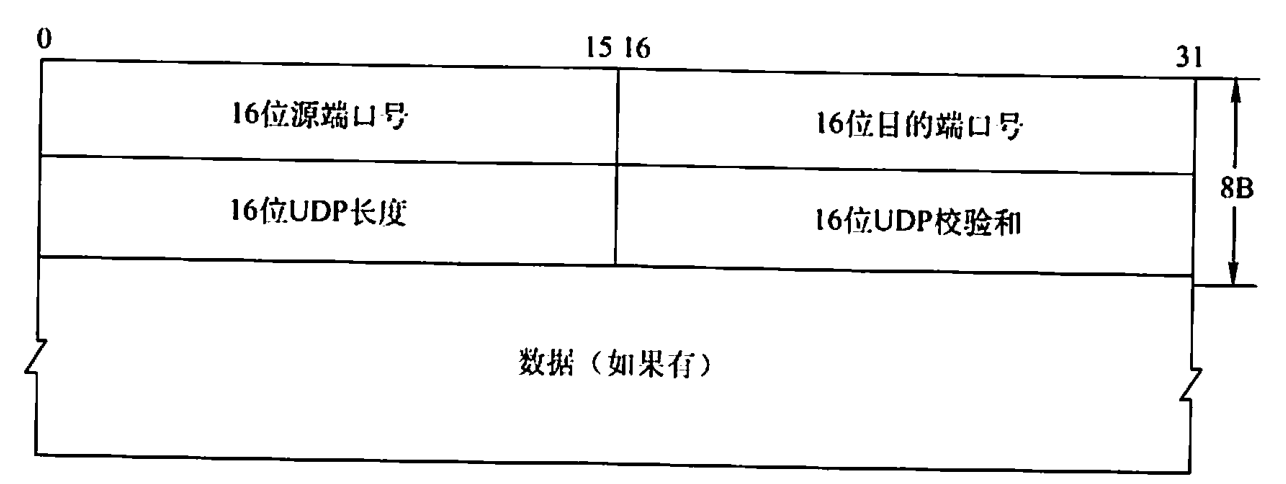
\includegraphics[width=0.8\textwidth]{./images/udp_header.png}
    \caption{UDP数据报的格式}
\end{figure}

UDP数据报=UDP首部+用户数据

UDP首部固定为8B长,分为4个字段,每个字段长度都是2B(16位)。
\begin{itemize}
    \item {\bf 源端口号}。如果不需要对方回信,可以设为全0。
    \item {\bf 目的端口号},必须指定。
    \item {\bf 长度}。指的是首部+数据部分的长度,最小值是8(即只有首部的情况)
    \item {\bf 校验和}。如果不希望进行校验,可以设为全0。
\end{itemize}

如果接收方发现报文中指定的端口号找不到对应的应用进程,就丢弃UDP数据报,并回传一个“端口不可达”的ICMP报文。

\subsubsection{UDP校验}

计算校验和时,需要在原本的首部前面加上12B的伪首部。这伪首部不参与发送,仅仅用于计算校验和。伪首部实际上是IP分组报头的一部分。

IP数据报的校验和只检验IP数据报的首部,而UDP的校验和则检验整个数据报。

如果数据部分不是偶数个字节长,则需要添加1个全0字节。

\subsection{TCP协议}

\subsubsection{TCP协议的特点}

\begin{itemize}
    \item 面向连接。TCP连接是一条逻辑连接。
    \item TCP是端到端的(进程到进程)
    \item 提供可靠交互服务,保证数据无差错、不丢失、不重复、不失序。
    \item 提供全双工通信,因此发送端和接收端都有发送和接收缓存。
    \item 面向字节流。
\end{itemize}

UDP报文的长度由应用进程决定,TCP报文的长度取决于接收方的接收窗口大小和网络的拥塞程度。

\subsubsection{TCP报文段}

TCP报文段=首部+数据

首部的前20B是固定的,如果需要,可以附加4N个字节的选项。

\begin{figure}[h]
    \centering
    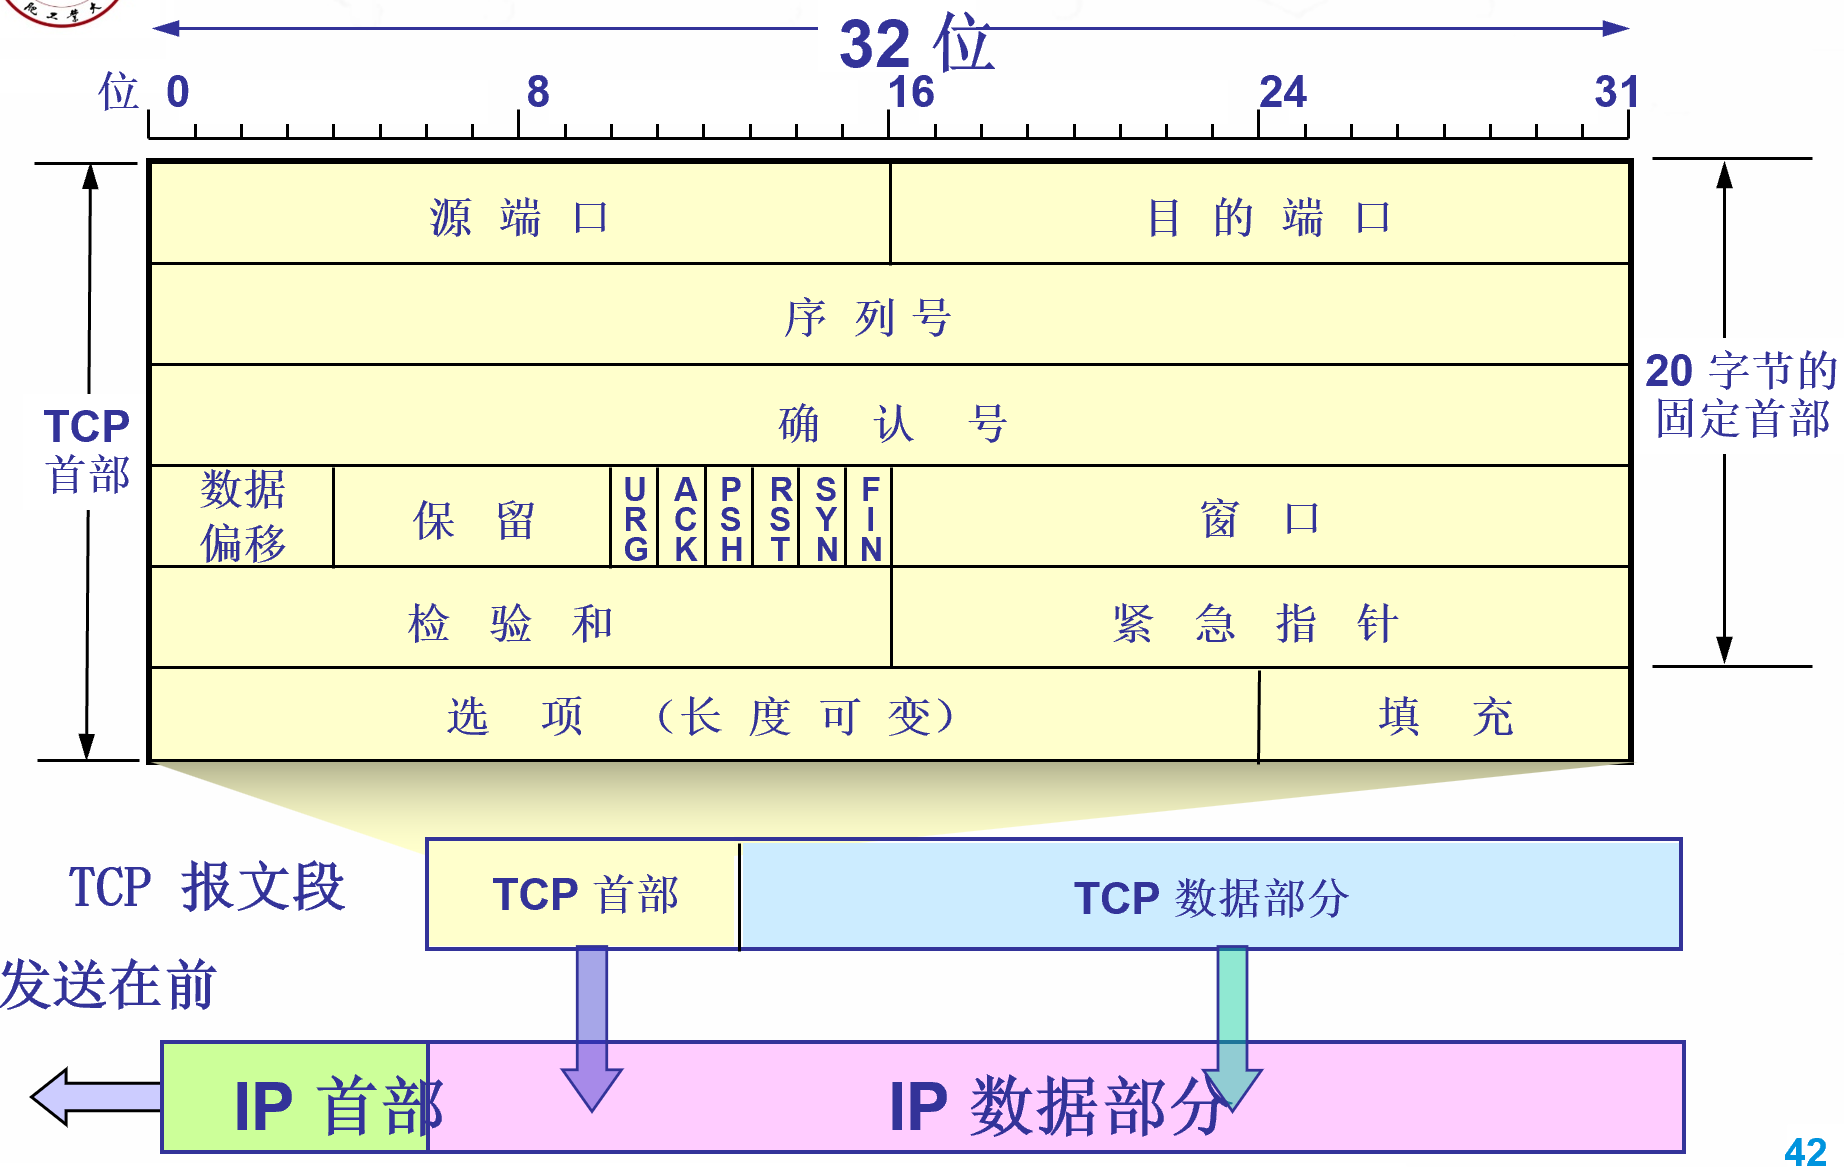
\includegraphics[width=0.7\textwidth]{./images/tcp_segment.png}
    \caption{TCP报文段的格式}
\end{figure}

\begin{itemize}
    \item {\bf 源端口和目的端口}。各占2B。
    \item {\bf 序号},占4B。指的是本报文段发送的数据的第一个字节的序号。
    \item {\bf 确认号},占4B。指的是\textbf{期望}收到下一个报文段的第一个数据字节的序号。若确认号为$N$,则表示到序号$N-1$为止的所有数据都已正确收到。
    \item {\bf 数据偏移},占4位。表示TCP首部的长度。这长度的单位是4B,由于4位二进制表示的最大值是15,因此TCP首部最长可以达到60B。
    \item {\bf 保留},占6位。目前恒为全0。
    \item {\bf 紧急位URG},和紧急指针字段配合使用。URG=1时,表示报文段中有紧急数据,需要尽快发送。
    \item {\bf 确认位ACK},仅当ACK=1时确认号才有效,否则确认号无效。建立TCP连接后,所有的报文段的ACK都等于1。
    \item {\bf 推送位PSH},接收方接收到PSH=1的报文段时,应当立即提交到应用层,而不是放在缓存里等待。
    \item {\bf 复位位RST},RST=1时,表示出现严重差错,必须断开TCP连接。
    \item {\bf 同步位SYN},SYN=1时表示这是一个连接请求或连接接受报文。
    \item {\bf 终止位FIN},用来释放TCP连接。FIN=1时,表明发送方要求释放连接。
    \item {\bf 窗口},占2B。表示当前允许对方发送的数据量。
    \item {\bf 校验和},占2B。和UDP一样,校验和校验的是整个报文段,且也要加上12B的伪首部(除协议字段从17改成6之外,其他和UDP伪首部完全一致)。
    \item {\bf 紧急指针},占2B。指出紧急数据有多少字节(紧急数据位于数据部分的最前面)。
    \item {\bf 选项},长度可变。
    \item {\bf 填充},仅仅是为了使首部长度是4B的整数倍。
\end{itemize}

\subsubsection{TCP连接管理}

每个TCP连接都有三个阶段:连接建立、数据传送和连接释放。

TCP连接采用C/S模式,主动发起连接的进程是Client,被动等待连接的进程是Server。

\begin{itemize}
    \item {\bf TCP连接的建立:三次握手}
    \begin{figure}[h]
        \centering
        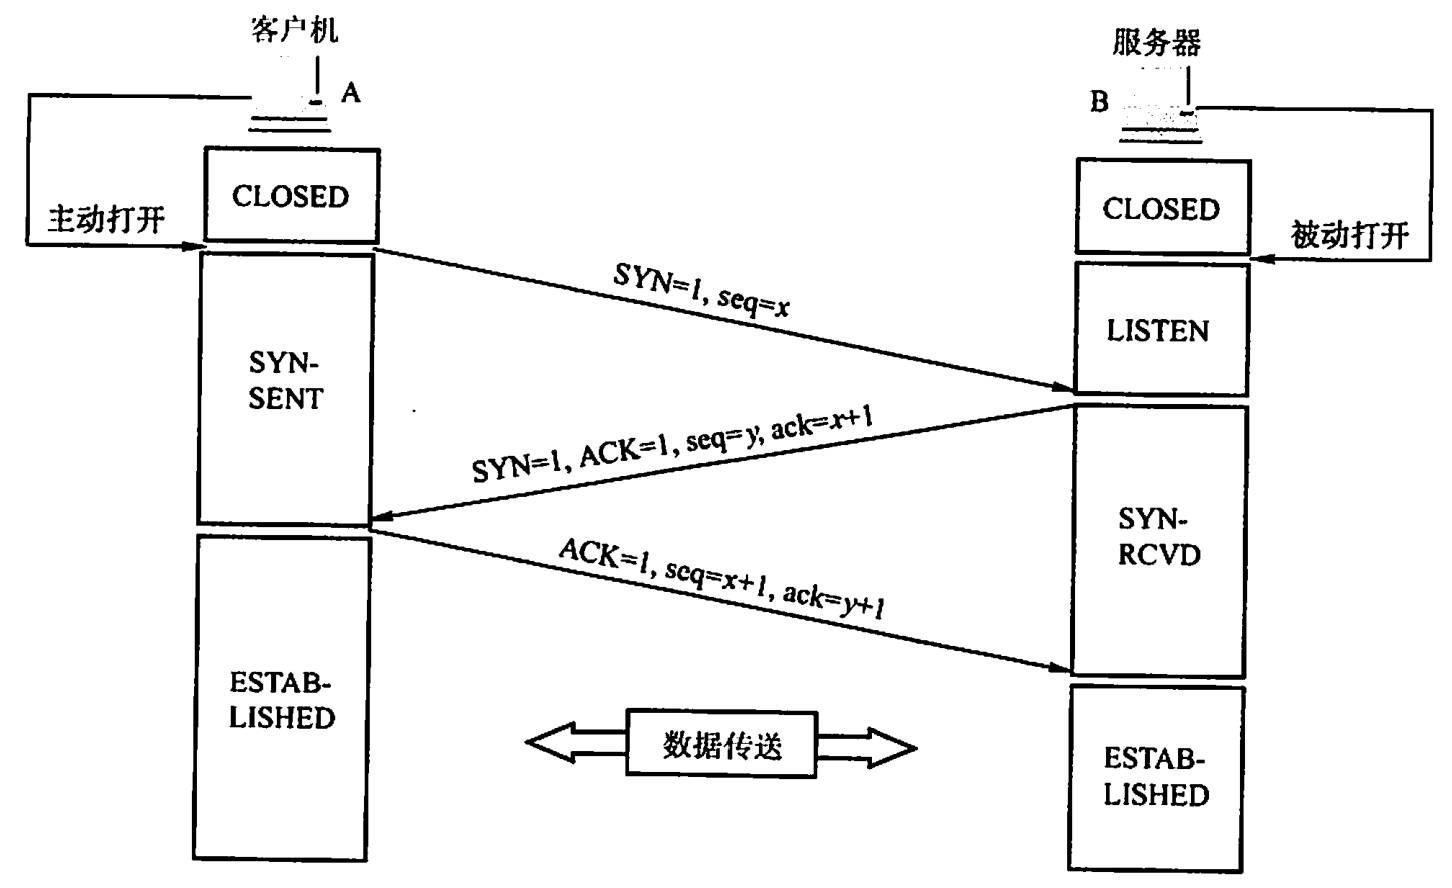
\includegraphics[width=0.7\textwidth]{./images/tcp_establish.png}
        \caption{三次握手过程}
        \label{tcp_establish}
    \end{figure}
    \begin{itemize}
        \item 第一步:客户机向服务器发送连接请求报文段,字段设置如图\ref{tcp_establish}所示。SYN报文段不能携带数据,但要消耗一个序号。此时TCP客户进程进入SYN-SENT状态。
        \item 第二步:服务器接收到请求后,如同意,则发回确认,并为连接分配响应的资源。字段设置如图\ref{tcp_establish}所示。确认报文段也不能携带数据、要消耗一个序号。此时TCP服务器进程进入SYN-RCVD状态。
        \item 第三步:客户机收到确认后,也要回传确认,并为连接分配响应的资源。字段设置如图\ref{tcp_establish}所示。此时,客户端进入ESTABLISHED状态。此报文段可以携带数据。
    \end{itemize}
    由于服务器先分配资源,客户端后分配资源,因此服务器容易受到SYN洪泛攻击。

    TCP连接一旦建立,再次尝试建立连接将会失败,原先的连接不受影响。
    \item {\bf TCP连接的释放:四次挥手}
    \begin{figure}[h]
        \centering
        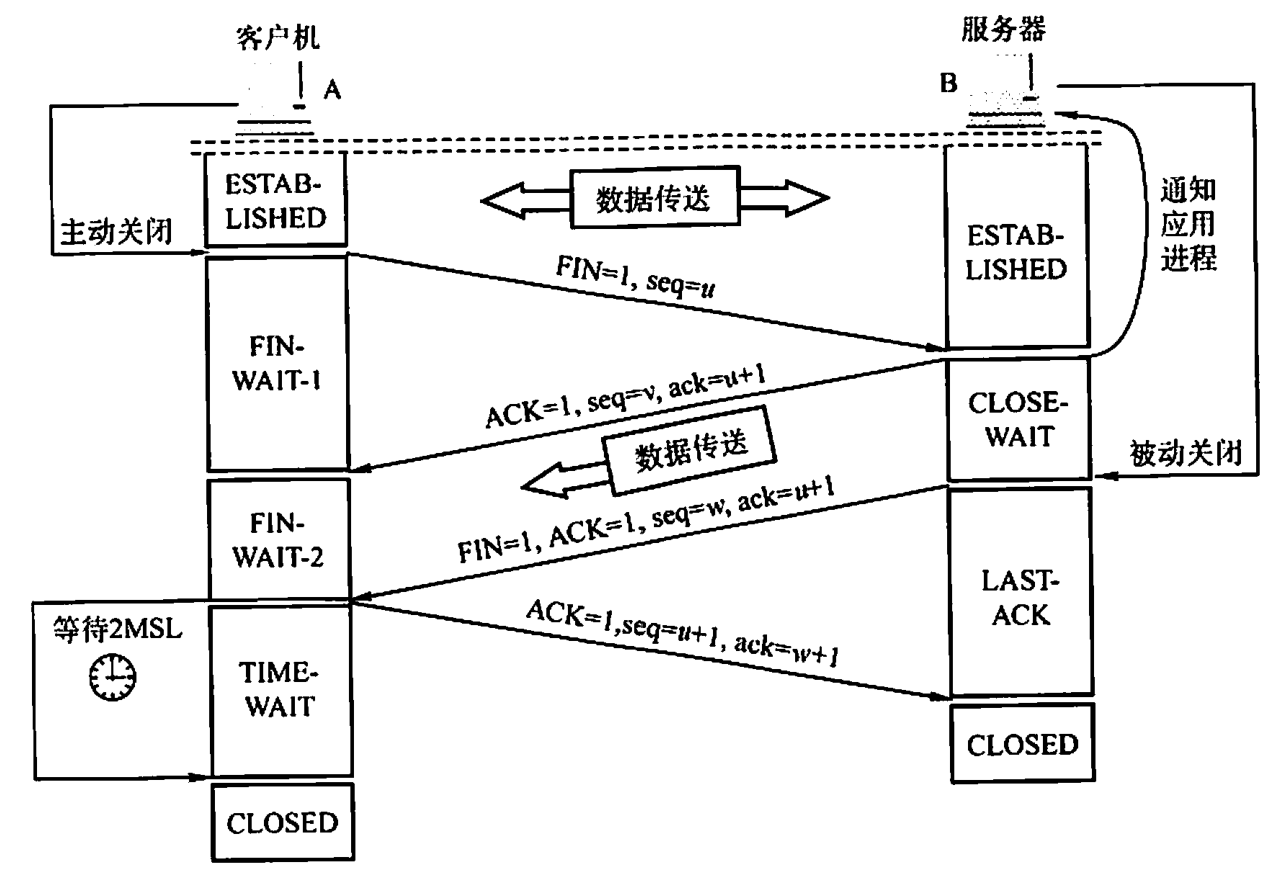
\includegraphics[width=0.7\textwidth]{./images/tcp_free.png}
        \caption{四次挥手过程}
    \end{figure}
    \begin{itemize}
        \item 第一步,客户机希望关闭连接时,发送一个FIN=1的报文段,进入FIN-WAIT-1状态。由于TCP是全双工的,此时对方仍然可以发送数据。
        \item 第二步,服务器收到连接释放报文后发回确认,进入CLOSE-WAIT状态。此时,从客户端到服务器这个方向的连接就已经释放,但服务器仍然可以继续发送数据。
        \item 第三步,服务器不需要再发送数据时,发出FIN=1的报文段,进入LAST-ACK状态。
        \item 第四步,客户机收到连接释放报文段后,发回确认,服务器收到确认后进入CLOSED状态。此时TCP连接还未释放,必须等待计时器超过2MSL后(此时认为网络中所有的报文都已到达目的地),客户机也进入CLOSED状态。
    \end{itemize}
\end{itemize}

\subsubsection{TCP可靠传输}

TCP使用校验、序号、确认和重传等机制来保证可靠连接。

TCP默认使用累积确认,即TCP只确认数据流中至第一个丢失字节为止的字节,即使丢失字节后面有正常接收的字节。

有两种事件会导致TCP对报文段进行重传:
\begin{itemize}
    \item 超时。TCP每发送一个报文段,就会重置一次计时器。如果计时器超时而仍未收到确认,就重传报文段。为了计算超时重传时间,TCP采用一种自适应算法(待补):
    \item 冗余ACK。TCP规定每当接收端收到比期望序号更大的报文段到达时,就发送一个冗余ACK信号,指明下一个期待字节的序号。如果接收端累计收到对同一个报文段的三个冗余ACK时,可以认为报文已经丢失,于是立即重传。这种技术通常称为\textbf{快速重传}。
\end{itemize}

\subsubsection{TCP流量控制}

TCP提供一种基于滑动窗口协议的的流量控制机制。在通信过程中,接收方根据自己接收缓存的大小,动态地调整发送方的发送窗口大小,这称为\textbf{接收窗口rwnd};同时,发送方根据其对网络拥塞程度的估计而切丁\textbf{拥塞窗口cwnd}的大小。

\subsubsection{TCP拥塞控制}

Internet建议标准定义了进行拥塞控制的4种算法:慢开始、拥塞避免、快重传和快恢复。

发送窗口的上限值是上节提到的接收窗口和拥塞窗口中较小的一个,即
\begin{equation*}
    \text{发送窗口的上限值}=\text{min}[\text{rwnd}, \text{cwnd}]
\end{equation*}

\begin{enumerate}
    \item 慢开始算法

    TCP连接刚刚建立时,先令拥塞窗口cwnd=1,即一个最大报文段长度MSS。每收到一个新的确认后,将cwnd加1,即增大一个MSS。

    需要注意当cwnd增加时,发送方一次可以发出更多报文段,则接收方的确认报文段也会增多,因此cwnd的增长速度会加快,从而呈现一种指数的趋势。所谓的“慢”指的不是cwnd增长慢,而是一开始限制cwnd到一个很小的值,从而使发送速率变得很慢。

    cwnd增大到一个规定的慢开始门限值ssthresh时,改用拥塞避免算法。具体来说,如果当前cwnd再次翻倍后超过了ssthresh,就将cwnd设为ssthresh,并改用拥塞避免算法。注意此时不能再翻倍cwnd了。
    \item 拥塞避免算法

    拥塞避免算法的思路是每经过一个RTT就让cwnd加1,而不是翻倍,这样cwnd将会按照线性增长。
    \begin{itemize}
        \item cwnd < ssthresh时,使用慢开始算法。
        \item cwnd > ssthresh时,使用拥塞避免算法。
        \item cwnd = ssthresh时,两种都可用,通常用拥塞避免算法。
    \end{itemize}
    无论在慢开始阶段还是拥塞避免阶段,只要检测到网络中出现拥塞,就立即把ssthresh设置为当前cwnd的一半(但不得小于2),同时将cwnd设置为1,重新执行慢开始。这样可以迅速减少主机发送的分组数量,给路由器争取出恢复的时间。
    \item 快重传

    快重传和快恢复算法都是对慢开始和拥塞避免算法的改进。

    冗余ACK也可用于网络拥塞的检测。当发送方连续收到三个重复的ACK报文时,直接重传对方尚未收到的报文段。
    \item 快恢复

    当发送方连续收到三个冗余ACK时,把ssthresh设置为此时发送方cwnd的一半,同时cwnd也减半(保持和ssthresh一致),然后执行\textbf{拥塞避免算法},而不是慢开始算法。这样发送速率恢复得较快,因此叫“快恢复”。
\end{enumerate}

注意本节为了简便,忽略了接收窗口rwnd,认为发送窗口只取决于拥塞窗口(cwnd)。实际上发送窗口是由rwnd和cwnd共同决定的。

\vspace{20pt}
超时重传时间(RTO)的确定对TCP的性能有重大影响。
\begin{itemize}
    \item 若RTO<RTT,则会造成很多不必要的重传;
    \item 若RTO$\gg$RTT,则会浪费资源,降低网络利用率。
\end{itemize}

RTT是一个动态更新的值,每个连接都有独立的RTT,且同一连接在不同时刻的RTT也可能不同。

TCP使用一个名为\textbf{加权平均往返时间RTT$_S$}的参数反映往返时间。一般来说,RTO应略大于RTT$_S$。

若是第一次测量到RTT样本,则RTT$_S$值就取为所测量到的RTT样本值;否则按照下式计算:
\begin{equation*}
    \text{新RTT}_S=(1-\alpha)\times\text{旧RTT}_S+\alpha\times\text{新RTT}_S\text{样本}
\end{equation*}
其中,$0\leq\alpha<1$。RFC 2988推荐的$\alpha$值为0.125。

RFC 2988建议使用下式计算RTO:
\begin{equation*}
    \text{RTO}=4\text{RTT}_S+4\times\text{RTT}_D
\end{equation*}
由此又引入RTT$_D$,若是第一次测量,RTT$_D$值取为测量到的RTT样本值的一半;否则,使用下式计算:
\begin{equation*}
    \text{新RTT}_D=(1-\beta)\times\text{旧RTT}_D+\beta\times\lvert\text{RTT}_S-\text{新RTT样本}\rvert
\end{equation*}
$\beta$的推荐值为0.25。

\section{应用层}

\subsection{网络应用模型}

\subsubsection{客户/服务器模型}

客户机是面向用户的,服务器是面向任务的。

\subsubsection{P2P模型}

与C/S模型相比,P2P模型的优点是:
\begin{itemize}
    \item 减轻了服务器压力,消除了对某个服务器的完全依赖,大大提高系统效率和资源利用率。
    \item 多个客户机之间可以直接共享文档。
    \item 可扩展性好。
    \item 网络健壮性强,单个节点故障不会对整体造成太大影响。
\end{itemize}

\subsection{域名系统(DNS)}

DNS系统采用C/S模型,运行在UDP之上,使用53号端口。

域名和IP地址并不是一一对应的关系。可以是一对一,也可以是一对多、多对一。

\begin{note}
    如果一台主机通过两张网卡接入两个网络,那么就具有两个IP地址。而一个域名可以映射到多台主机(负载均衡),一台主机也可以映射到多个域名(虚拟主机)。
\end{note}

\subsubsection{域名服务器}

DNS使用了大量的域名服务器,它们以层次方式组织起来。这是典型的分布式系统。域名服务器有如下4种:
\begin{enumerate}
    \item {\bf 根域名服务器}。层次最高。根域名服务器知道所有顶级域名服务器的IP地址。本地域名服务器如果无法解析域名,就要咨询根域名服务器。世界上有13个互为备份的根域名服务器。
    \item {\bf 顶级域名服务器}。管辖在该顶级域名(如.com)下注册的所有二级域名。
    \item {\bf 授权域名服务器},又叫权限域名服务器。每台接入互联网的主机都必须在授权域名服务器处登记,可以登记不止一台。
    \item {\bf 本地域名服务器}。一台主机发出DNS查询请求时,就是本地域名服务器响应了请求。
    
    实际上,很多服务器都同时充当了后两者。
\end{enumerate}

\subsubsection{域名解析过程}

域名解析可以是正向解析(域名->IP地址),也可以是反向解析(IP地址->域名)。

域名解析有两种方式:递归查询和递归与迭代相结合的查询。
\begin{enumerate}
    \item 主机向本地域名服务器的查询采用递归查询。
    \item 本地域名服务器向根域名服务器的查询采用迭代查询。
\end{enumerate}

\begin{problem}
    假设某主机访问访问连接http://www.abc.com/index.html,局域网内的本地域名服务器为递归查询,其他所有域名服务器为迭代查询,局域网访问外网的时延不可忽略,其他各种时延均可忽略,则从点击超链接到浏览器接收到index.html为止,可能的最短RTT和最长RTT分别是(\ \ )和(\ \ )。
\end{problem}
\begin{solution}
    2, 5
    \begin{itemize}
        \item 最理想情况:主机有www.abc.com到其IP地址的映射缓存,无需DNS查询,直接请求文件,则TCP连接建立需要一个RTT,请求文件需要一个RTT。
        \item 最坏情况:主机向本地域名服务器查询www.abc.com的IP地址(延时忽略),本地域名服务器迭代查询,访问根域名服务器、.com顶级域名服务器、abc.com域名服务器,分别花费1个RTT,共3个RTT,再加上上述的2个RTT,为5RTT。
    \end{itemize}
\end{solution}

\subsection{文件传输协议(FTP)}

FTP允许客户指明文件的类型与格式,并允许文件具有存取权限。

FTP服务器分为两部分:
\begin{itemize}
    \item 一个主进程,负责接收新的请求。
    \item 若干个从属进程,负责处理单个请求。
\end{itemize}

FTP的连接也分两种:
\begin{itemize}
    \item 控制连接,监听21端口
    \item 数据连接,监听20端口
\end{itemize}

文件列表是通过数据连接传送的。

\subsection{电子邮件}

\subsubsection{电子邮件系统的组成结构}

一个电子邮件系统应具有三个主要组成构件:
\begin{itemize}
    \item {\bf 用户代理(UA)}。用户和电子邮件系统的接口。通常情况下就是电子邮件客户端软件。
    \item {\bf 邮件服务器}。负责发送和接收文件,采用C/S模式工作,但一个邮件服务器必须能够同时充当客户端和服务器。
    \item {\bf 邮件发送和读取协议}。如SMTP和POP3(或IMAP)。SMTP是“推”的方式,POP3是“拉”的方式。
\end{itemize}

POP3在传输层使用明文传送密码。

\subsection{万维网(WWW)}

\subsubsection{超文本传输协议 HTTP}

HTTP包含两类报文:
\begin{itemize}
    \item 请求报文
    \item 响应报文
\end{itemize}

HTTP本身是无连接的,即虽然HTTP基于TCP,但通信双方在通信之前无需建立HTTP连接。

HTTP是无状态的。服务器不记得是否为某一特定主机服务过,也不记得服务过多少次。(但是可以通过Cookie+数据库的方式跟踪用户的活动)

HTTP可以使用非持久连接,也可以使用持久连接(HTTP/1.1支持)
\begin{itemize}
    \item 非持久连接下,每个网页元素对象都需要建立并释放一次TCP连接,请求一个WWW文档需要的时间=该文档的传输时间+两倍RTT(TCP建立一倍,请求和接收文档一倍)
    \item 持久连接下,一个TCP连接上可以多次传送HTTP报文。又分流水线和非流水线两种方式:
    \begin{itemize}
        \item 非流水线方式:客户在收到前一个响应后才能发出下一个请求,浪费资源。
        \item 流水线方式:可以连续发请求。
    \end{itemize}
\end{itemize}

HTTP/1.1默认使用流水线的持久连接。

\subsection{应用层协议总结}

\begin{table}[h]
    \centering
    \resizebox{\linewidth}{!}{
        \begin{tabular}{c|c|c|c|c|c|c|c|c|c}
            \hline
            应用程序 & FTP数据连接 & FTP控制连接 & TELNET & SMTP & DNS & TFTP & HTTP & POP3 & SNMP \\
            \hline
            使用协议 & TCP & TCP & TCP & TCP & UDP & UDP & TCP & TCP & UDP \\
            \hline
            熟知端口号 & 20 & 21 & 23 & 25 & 53 & 69 & 80 & 110 & 161 \\
            \hline
        \end{tabular}
    }
    \caption{常见应用层协议小结}
\end{table}

\end{document}